%&pdfLaTeX
% !TEX encoding = UTF-8 Unicode
\documentclass{article}
\usepackage{ifxetex}
\ifxetex
\usepackage{fontspec}
\setmainfont[Mapping=tex-text]{STIXGeneral}
\else
\usepackage[T1]{fontenc}
\usepackage[utf8]{inputenc}
\fi
\usepackage{textcomp}

\usepackage{graphicx}
\usepackage{array}
\usepackage{ulem}
\usepackage{amssymb}
\usepackage{fancyhdr}
\renewcommand{\headrulewidth}{0pt}
\renewcommand{\footrulewidth}{0pt}
\usepackage{color}

\pagestyle{fancy}
\rhead{}
\rfoot{}
\chead{}
\cfoot{}
\fancyfoot[LO]{
 Draft ... \thepage{}}
\definecolor{color02}{rgb}{0.00,0.00,1.00}

\begin{document}

\vspace{72pt}
\section*{{\LARGE{}\textbf{LatihanVSPsu}}}

\vspace{24pt}
VSP Processing Exercise using Seismic Unix

\vspace{12pt}
fahdi@gm2001.net

\vspace{12pt}
February 2012

\vspace{24pt}
\textbf{DESCRIPTION}

\vspace{24pt}
Set of script to model and process simple geometry/simple vertical seismic profiling 
(VSP) data. This document also explained basic understanding about VSP (acquisition, 
processing, and application/interpretation).

\vspace{24pt}
\textbf{REQUIREMENT }

\vspace{12pt}
- Basic understanding of Unix/Linux command and shell scripting would be advantage 
in learning this. 

\vspace{12pt}
- Seismic Unix (http://www.cwp.mines.edu/cwpcodes/)

\vspace{12pt}
- Ela2D (Get copy at http://www.gm2001.net/latihanvspsu/)\fancyfoot[LO]{\thepage{}}
\newpage

\newpage
\vspace{72pt}
\textbf{SOURCE CODE REPOSITORY}

\vspace{24pt}
I put repository on github

\vspace{12pt}
{\color{color02} \emph{https://www.github.com.fahdi104/latihanvspsu}}

\vspace{24pt}
If you have git account, you can fork this by typing

\vspace{12pt}
\$git clone {\color{color02} \emph{git@github.com:fahdi104/latihanvspsu.git}}

\vspace{24pt}
I will also publish to 

\vspace{12pt}
{\color{color02} \emph{http://www.gm2001.net/latihanvspsu}}

\vspace{24pt}
Please join me to develop this script or update/edit this document. 

\vspace{24pt}
\textbf{DATASET FOR EXERCISE}

\vspace{24pt}
The dataset used for this exercise and displayed in this documents was using Naylor-1 
well, available for research from Earth Resources, Dept. of Primary Industries, 
State Government of Victoria Australia. 

\vspace{12pt}
({\color{color02} \emph{http://er-info.dpi.vic.gov.au/petroleum/assets/pe91072.htm\#pe910726}}) 
or contact them directly for information of the data.

\vspace{24pt}
\textbf{Document Version}

\vspace{12pt}
Version 0.1  February 2012

\vspace{12pt}
Version 0.2 April 2013\newpage

\newpage
\vspace{36pt}
\section*{{\LARGE{}\textbf{VSP Overview}}}

\vspace{24pt}
Vertical seismic profiling (VSP) or in general known as borehole seismic, is a 
kind of seismic survey where put the seismic receiver inside a wellbore (as opposed 
to surface seismic where we put the receiver on surface), and generated the source 
from surface (or from wellbore, depend on the configuration). This kind of survey 
is generally part of wellbore characterization (well-logging), combined with other 
logging methodology to extract information from a wellbore such as radioactive 
logging (gamma ray, density, and neutron), sonic logging etc.

\vspace{24pt}
Main purpose of running VSP survey is to get time and depth relation. Using wireline 
cable we can measure the depth, and by shooting seismic wave from surface we can 
measure what is the transit time of the seismic wave to the receiver at certain 
depth. This time-depth relation will be used to relate log data in depth with seismic 
data in time, and further to build velocity model for depth to time or time to 
depth conversion of subsurface model. 

\vspace{24pt}
VSP survey normally defined by the type of source configuration that used in the 
acquisitions, because the receiver is always fixed inside the wellbore. For example 
if we are using single source with fixed offset close to well (receiver), this 
survey known as zero offset VSP. If we have fixed offset that relatively far away 
from wellbore, this can be near offset VSP survey or far offset VSP survey. In 
a case of multi offset VSP, where we shot directly above VSP receiver (particularly 
for deviated well), this survey known as walkabove VSP or vertical incidence VSP. 
And if we shot in multi offset within particular direction away from the wellbore, 
this is known as multi offset walkaway VSP. If we shot quite dense in 3D, this 
is known as 3D VSP. 

\vspace{24pt}
Choices of which VSP survey/data that we want to acquire will be depend on what 
is the objective that we want to achive. If we only want to get time-depth relation 
and 1-D seismic image for correlation we can utilized zero offset VSP. In case 
we want to get structural image, we can used near offset, far offset, or multi 
offset walkaway VSP. If we required to measured anisotropic response in the borehole 
we need to run multi offset Walkaway VSP. Normally for complex VSP survey (more 
than zero offset VSP), it is required to run pre-survey modeling either by simple 
ray tracing to check illumination coverage or by doing full waveform modeling to 
see feasibility of recorded data to achieve the required objectives.  

\vspace{24pt}
The processed full VSP waveforms can output 1-D or 2-D (or even 3-D) seismic image 
in the borehole. Theoretically VSP image is higher in resolution due to shorter 
raypath compare to surface seismic. And VSP imaging is controlled in depth, therefore 
provide more accurate depth image information. Furthermore than corridor stacks, 
depending on survey configuration, VSP can be utilized further for look ahead-depth 
predictions, structural imaging, attenuation factor estimations, and anisotropy 
parameter estimations.

\vspace{24pt}
Operational wise, VSP can be run on open hole or cased hole wellbore. In the acquisitions, 
normally VSP is part of logging sequence that came last (because it's can be run 
in open hole and cased hole), and it can be run for the whole sections. There are 
two main components for VSP logging operation, downhole tools that are the receiver 
(geophone), and surface equipment which consist of seismic source and surface seismic 
sensors to QC the source. The data quality will be depend on how good the wellbore 
condition, and the coupling of receiver with the formations.  In cased hole (dual 
casing or even triple casing) environment this will also depend on the cement integrity 
between casing. And of course the data quality will also depend whether the source 
is working properly to generate seismic source or not. 

\vspace{24pt}
Borehole seismic downhole tools (receiver/geophone) are generally a multicomponent 
geophone, record data in horizontal (X-Y component) and vertical component (Z). 
The tools can be conveyed using wireline cable, tractor, or nowadays inside a drilling 
tools component for seismic while drilling operations. The source itself can be 
an airgun that generates pressure, in land operation this gun was put inside a 
gun pit filled with water, and can be attached in boat for offshore operations. 
Vibroseis is also common to used for VSP survey, especially in desert area. 

\vspace{24pt}
In borehole seismic data, there are two important wave. These wave was divived 
by the way the recorded in receiver, the first wave are downgoing waves that is 
wave that travels directly from seismic source to the receiver. This wave measure 
direct P waves transit time which further more used for time-depth information. 
The second type of the wave is the upgoing wave or the reflection waves. These 
wave travels from source hitting formation, reflected back and recorded at the 
receiver. Depending on formation properties, and the type of source, downgoing 
and upgoing can be consist of compressional wave (P wave) and also shear waves 
(S wave) , that is downgoing P, downgoing S, upgoing P, and upgoing S. The reflection 
wave is the one that is required for subsurface imaging in borehole seismic. The 
exercise for modeling these various wavetype can be seen in the Synthetic Elastic 
Modeling chapter. 

\vspace{24pt}
The understanding of various wave type within borehole seismic data is fundamental 
in order to be able to process, analyze, and interpret VSP data. For example, we 
need to know which one that we need for time-depth informations, and anisotropy 
parameter inversion. This is the direct wave in zero offset VSP for time depth 
informations, and direct wave in multi offset walkaway VSP survey for anisotropy 
parameter inversion. For structural imaging we required to identify and separate 
the reflection wave, and this is also depend whether we want to image using P wave 
or S wave. Besides the primary wave (primary downgoing, and primary reflections) 
it is also useful if we can estimate the multiple. 

\vspace{24pt}
Just like any other seismic method, the way we processed the VSP data is more or 
less the same. At least there are five mandatory steps in processing borehole seismic 
data for any kind of survey. First step is to break time picking, because this 
is the basis of any kind of the subsequence processing. This is crucial steps, 
because from this step we define the velocity model for separation, imaging, etc. 
Second step is preconditioning the data; this is will be subject to tools and condition 
that we faced. In example when we processed vectorial data (X-Y-Z), we required 
to polarize and project the data to 2-D frame or 3-D frame to get true horizontal 
and true vertical data. And if we required compensating for spherical divergence 
or statistical variation because of tools in data or when we required removing 
unwanted frequency. Third steps is wavefield separations, this is also crucial 
that we extract the type of wave that we want for further analyzed. Normally we 
try to maximize in extracting the best possible of reflection wave from the total 
wavefield data. Next mandatory steps is deconvolutions, because we want to remove 
the multiple. The final steps is imaging, whether we are going to extract 1-D seismic 
profile for corridor stacks, or using CDP mapping or migration to get 2-D/3-D image. 

\vspace{36pt}
\section*{{\LARGE{}\textbf{Latihan VSP SU Scripts}}}

\vspace{24pt}
The directory is numbered in a way to sequentially exercise VSP modeling and processing. 
You can start with directory number 1 (BuildFlatModel) if you want to start with 
synthetic data processing. Or if you already have field SEGY data, you can start 
with directory number 0 (ImportSEGY). 

\vspace{24pt}
\subsection*{\textbf{File Index}{\large{}\textbf{File List}}}

\vspace{12pt}
Here is a list of all documented files with brief descriptions:

\vspace{1pt}
\leftskip=18pt
\textbf{0ImportSEGY/ImportSEGY.sh (Convert SEGY to SU format, setting required 
VSP headers )}  \pageref{AAAAAAAAAB}

\vspace{1pt}
\textbf{1BuildFlatModel/CreateFlatModel.sh (Create Simple Flat Model )}  \pageref{AAAAAAAAAC}

\vspace{1pt}
\textbf{2Ela2D/CreateElasticSynthetic.sh (Do elastic synthetic modeling using ela2d 
)}  \pageref{AAAAAAAAAE}

\vspace{1pt}
\textbf{3BreakTimePick/FBAutoPick.sh (Automatic FB picking )}  \pageref{AAAAAAAAAI}

\vspace{1pt}
\textbf{4Preprocessing/FrequencyAnalysis.sh (Create FZ Spectrum \& FK-Spectrum 
)}  \pageref{AAAAAAAAAJ}

\vspace{1pt}
\textbf{4Preprocessing/Preprocessing.sh (Do Preprocessing: BPF, Normalize, TVG 
)}  \pageref{AAAAAAAAAK}

\vspace{1pt}
\textbf{5Separation/Separation.sh (Run wavefield separation based on TT using median 
velocity filter )}  \pageref{AAAAAAAAAM}

\vspace{1pt}
\textbf{6Deconvolution/ApplyDecon.sh (Apply PEF to upgoing wavefield )}  \pageref{AAAAAAAAAN}

\vspace{1pt}
\textbf{6Deconvolution/CheckAutoCorrelation.sh (Check auto correlation to determine 
optimum lag and prediction on downgoing wavefield )}  \pageref{AAAAAAAAAO}

\vspace{1pt}
\textbf{7CorrStack/CorridorStack.sh (Create corridor stack )}  \pageref{AAAAAAAAAP}\newpage

\newpage
\vspace{24pt}
\section*{{\LARGE{}\textbf{File DocumentationFile Documentation}}}

\vspace{12pt}
\subsection*{{\large{}\textbf{0ImportSEGY/ImportSEGY.sh File Reference}}}

\vspace{12pt}
\leftskip=0pt
20ImportSEGY/ImportSEGY.sh0ImportSEGY/ImportSEGY.sh\label{AAAAAAAAAB}

\vspace{12pt}
Convert SEGY to SU format, setting required VSP headers. 

\vspace{24pt}
\subsubsection*{\textbf{Detailed Description}}

\vspace{1pt}
The purposes of this script are to convert field VSP SEGY to SU format, and also 
set a few parameters that is required in further processing. 

\vspace{1pt}
Currently it is tested for Schlumberger VSI* field SEGY. 

\vspace{1pt}
Most important header for VSP is receiver depth. And if also possible other field 
recording information such as acquisition shot number, acquisition shot time, also 
field transit time picks. 

\vspace{4pt}
\textbf{Usage:}

\vspace{4pt}
Open the file in text editor, and edit required parameters as necessary. The parameter 
description is given here. Run the command from console. 

\vspace{16pt}
\$./ImportSEGY.sh 

\vspace{4pt}
\textbf{Output:}

\vspace{4pt}
- SU File 

\vspace{4pt}
- Transit Time Header and Receiver Depth in ASCII format (currently tested for 
SLB VSI SEGY)

\vspace{4pt}
\textbf{Parameters:}

\vspace{4pt}
\begin{tabular}{|>{\raggedright}p{54pt}|>{\raggedright}p{245pt}|}
\hline
i\textit{nput}  & Specify your input SEGY file \tabularnewline
\hline
o\textit{utput}  & Specify your output SU file \tabularnewline
\hline
t\textit{min}  & Minimum Output time \tabularnewline
\hline
t\textit{max}  & Maximum Output time \tabularnewline
\hline
\end{tabular}

\vspace{4pt}
\textbf{Author:}

\vspace{4pt}
\leftskip=18pt
fahdi@gm2001.net 

\vspace{4pt}
\leftskip=0pt
\textbf{Date:}

\vspace{4pt}
\leftskip=18pt
February 2012 \pagebreak{}

\vspace{16pt}
\leftskip=0pt
\textbf{Script Source:}

\vspace{4pt}
Filename: ImportSEGY.h

\vspace{16pt}
00001 \#!/bin/bash\label{l00002}

\vspace{4pt}
00002 \label{l00015}

\vspace{4pt}
00015 \# Input\label{l00016}

\vspace{4pt}
00016 input=VSI\_007\_A\_gac\_wavefield\_z\_resize.sgy\label{l00017}

\vspace{4pt}
00017 output=realZ.su\label{l00018}

\vspace{4pt}
00018 \label{l00019}

\vspace{4pt}
00019 \# set parameter\label{l00020}

\vspace{4pt}
00020 tmin=0 \#start time\label{l00021}

\vspace{4pt}
00021 tmax=4 \#output time\label{l00022}

\vspace{4pt}
00022 \label{l00023}

\vspace{4pt}
00023 segyread tape=\$input verbose=1 endian=0 \textbar{} suwind tmin=\$tmin tmax=\$tmax 

\vspace{4pt}
\texttt{>} \$output.tmp1\label{l00024}

\vspace{4pt}
00024 \label{l00025}

\vspace{4pt}
00025 \#housekeeping, just to make output SU available for XWIGB\label{l00026}

\vspace{4pt}
00026 \#this is not a good practice, because I have to strip SEGY headers, 

\vspace{4pt}
will think about this later\label{l00027}

\vspace{4pt}
00027 sugethw \texttt{<} \$output.tmp1 key=lagb,gelev \textbar{} sed -e 's/unscale=//' 
-e 

\vspace{4pt}
's/gelev=//' -e 's/lagb=//'\textbar{} sed '/\textasciicircum{}\$/d' \texttt{>} 
tt-header.tmp\label{l00028}

\vspace{4pt}
00028 awk '\{ printf \texttt{"}\%4f \%d\textbackslash{}n\texttt{"}, \$1/1000, \$2/10000 
\}' tt-header.tmp \texttt{>} tt-

\vspace{4pt}
header.txt\label{l00029}

\vspace{4pt}
00029 \label{l00030}

\vspace{4pt}
00030 awk '\{print \$2\}' tt-header.txt \textbar{} a2b \texttt{>} gelev.bin\label{l00031}

\vspace{4pt}
00031 sushw \texttt{<} \$output.tmp1 key=d1,scalel,scalco \texttt{>} \$output.tmp2\label{l00032}

\vspace{4pt}
00032 sushw \texttt{<} \$output.tmp2 key=gelev infile=gelev.bin\texttt{>} \$output\label{l00033}

\vspace{4pt}
00033 \label{l00034}

\vspace{4pt}
00034 \#display\label{l00035}

\vspace{4pt}
00035 nrec=(\$(wc -l tt-header.txt \textbar{} awk '\{print \$1\}'))\label{l00036}

\vspace{4pt}
00036 \label{l00037}

\vspace{4pt}
00037 suxwigb \texttt{<} \$output title=\$input perc=97 style=vsp key=gelev 

\vspace{4pt}
curve=tt-header.txt npair=\$nrec,1 curvecolor=red \&\label{l00038}

\vspace{4pt}
00038 \label{l00039}

\vspace{4pt}
00039 \#clean up\label{l00040}

\vspace{4pt}
00040 rm *.tmp*\label{l00041}

\vspace{4pt}
00041 rm *.bin\label{l00042}

\vspace{4pt}
00042 \newpage

\newpage
\vspace{12pt}
\subsection*{{\large{}\textbf{1BuildFlatModel/CreateFlatModel.sh File Reference}}}

\vspace{12pt}
21BuildFlatModel/CreateFlatModel.sh1BuildFlatModel/CreateFlatModel.sh\label{AAAAAAAAAC}

\vspace{12pt}
Create Simple Flat Model. 

\vspace{24pt}
\subsubsection*{\textbf{Detailed Description}}

\vspace{1pt}
In this folder we will exercise how to create flat model using unif2 from SU. For 
simple zero offset VSP, flat model should be sufficient. This scripting is also 
preparing the required file for Ela2D modeling, such as Vp, Vs, and density file 
in binary format.

\vspace{1pt}
Within this exercise we will also generate shooting geometry that we will use for 
next exercise in building synthetic data.Clean.sh can be used to clean up Model 
can be displayed by typing ./DisplayModel.sh

\vspace{1pt}
It's also good practice to see unif2 manual. 

\vspace{1pt}
Clean.sh is used to delete exercise's output file.

\vspace{4pt}
\textbf{Usage:}

\vspace{4pt}
Open the file in text editor, and edit required parameters as necessary. The parameter 
description is given here. Run the command from console. 

\vspace{16pt}
\$./CreateFlatModel.sh 

\vspace{4pt}
\textbf{Output:}

\vspace{4pt}
- Vp, Vs, and Density in binary format (automatically copied to 2Ela2D directory)

\vspace{4pt}
- Source \& Receiver Listing in ASCII format (table: depth - offset)

\vspace{16pt}
\textbf{Parameters:}

\vspace{4pt}
\textit{nx} Number of model sample in X direction 

\vspace{4pt}
\begin{tabular}{|>{\raggedright}p{54pt}|>{\raggedright}p{245pt}|}
\hline
\tabularnewline
\hline
d\textit{x}  & Model sampling rate in X direction \tabularnewline
\hline
n\textit{z}  & Number of model sample in Z direction \tabularnewline
\hline
d\textit{z}  & Model sampling rate in Z direction \tabularnewline
\hline
w\textit{hx}  & Wellhead location X \tabularnewline
\hline
w\textit{hy}  & Wellhead location Y \tabularnewline
\hline
r\textit{cv\_x}  & Receiver location X \tabularnewline
\hline
r\textit{cv\_spacing}  & Receiver Spacing \tabularnewline
\hline
r\textit{cv\_z0}  & Depth of first receiver \tabularnewline
\hline
n\textit{rcv}  & Number of Receiver \tabularnewline
\hline
o\textit{ffset}  & Source Offset from wellhead \tabularnewline
\hline
s\textit{rc\_z}  & Depth of source \tabularnewline
\hline
n\textit{inf}  & Number of interface in unif2 model \tabularnewline
\hline
V\textit{p}  & P velocity for each layers \tabularnewline
\hline
V\textit{s}  & S velocity for each layers \tabularnewline
\hline
d\textit{ensity}  & Density for each layers \tabularnewline
\hline
\end{tabular}

\vspace{1pt}
Definition in file \textbf{CreateFlatModel.sh}.

\vspace{4pt}
\textbf{Author:}

\vspace{4pt}
\leftskip=18pt
fahdi@gm2001.net 

\vspace{4pt}
\leftskip=0pt
\textbf{Date:}

\vspace{4pt}
\leftskip=18pt
February 2012 

\vspace{16pt}
\leftskip=0pt
\textbf{Output Example:}

\vspace{4pt}
\$./DisplayModel.sh

\vspace{16pt}
%%\begin{figure}[htbp]
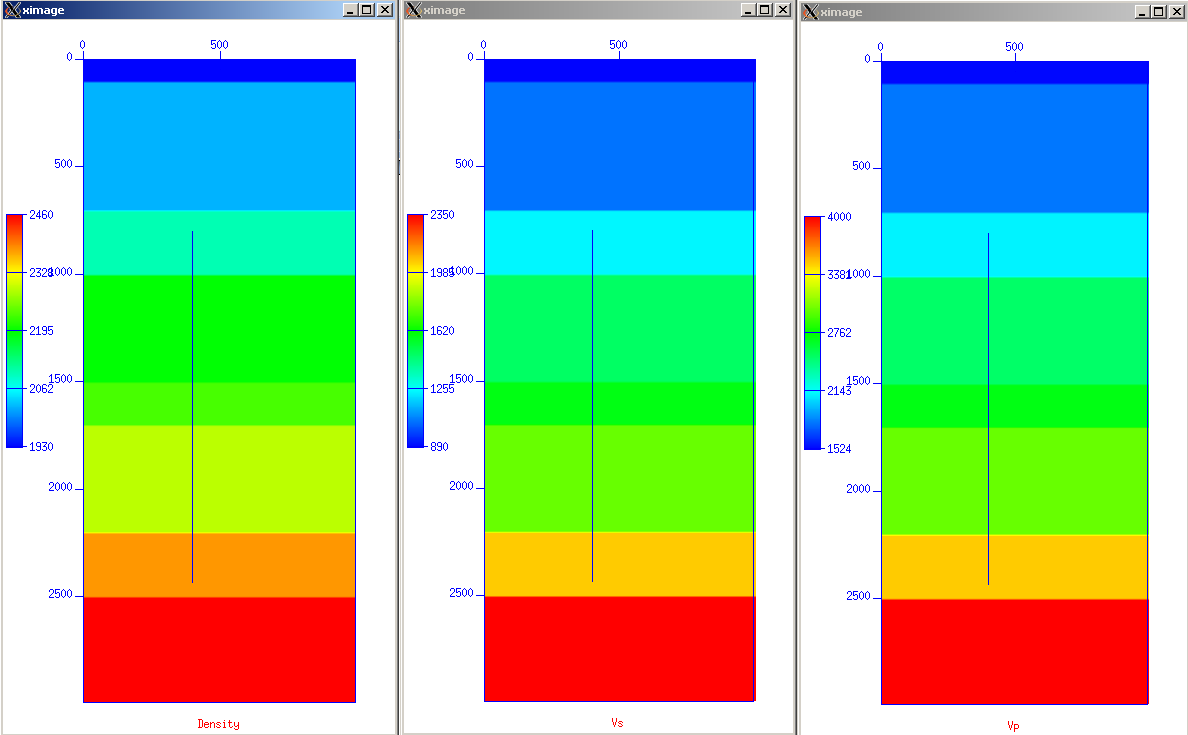
\includegraphics[width=463pt, height=287pt, keepaspectratio=true]{LatihanVSPsu-fig001.png}
%%\caption{This should be the caption for \texttt{LatihanVSPsu-fig001.png}.}
%%\end{figure}

\pagebreak{}

\vspace{28pt}
\textbf{Script Source:}

\vspace{4pt}
Filename: CreateFlatModel.sh

\vspace{4pt}
00001 \#!/bin/bash

\vspace{4pt}
00002 

\vspace{4pt}
00028 \#input

\vspace{4pt}
00029 \#define model dimension

\vspace{4pt}
00030 nx=100

\vspace{4pt}
00031 dx=10

\vspace{4pt}
00032 nz=300

\vspace{4pt}
00033 dz=10

\vspace{4pt}
00034 

\vspace{4pt}
00035 

\vspace{4pt}
00036 \#set parameter

\vspace{4pt}
00037 \#Define Shooting Geometry

\vspace{4pt}
00038 \#wellhead location which will be receiver location

\vspace{4pt}
00039 whx=400

\vspace{4pt}
00040 why=0

\vspace{4pt}
00041 

\vspace{4pt}
00042 \#receiver\label{l00043}

\vspace{4pt}
00043 rcv\_x=\$((whx))\label{l00044}

\vspace{4pt}
00044 rcv\_spacing=15\label{l00045}

\vspace{4pt}
00045 rcv\_z0=800 \label{l00046}

\vspace{4pt}
00046 nrcv=110\label{l00047}

\vspace{4pt}
00047 \label{l00048}

\vspace{4pt}
00048 \#source, set by offset from wellhead\label{l00049}

\vspace{4pt}
00049 offset=100\label{l00050}

\vspace{4pt}
00050 src\_z=50\label{l00051}

\vspace{4pt}
00051 \label{l00052}

\vspace{4pt}
00052 \label{l00053}

\vspace{4pt}
00053 \#We will create model where interface defined by \$input\_model, contain 

\vspace{4pt}
8 layer\label{l00054}

\vspace{4pt}
00054 \#change the velocity for interface here\label{l00055}

\vspace{4pt}
00055 \#To simply the exercise set Vp/Vs=2, and density is gardner\label{l00056}

\vspace{4pt}
00056 \#output name is designed for Ela2d (vel\_P.dat, vel\_S.dat, density.dat)\label{l00057}

\vspace{4pt}
00057 \#see SU documentation for unif2  to modify\label{l00058}

\vspace{4pt}
00058 \label{l00059}

\vspace{4pt}
00059 input\_model=model.unif2\label{l00060}

\vspace{4pt}
00060 ninf=8 \#number of interface, check with \$input\_model\label{l00061}

\vspace{4pt}
00061 Vp=1524,1800,2100,2500,2700,3000,3500,4000 \#m/s\label{l00062}

\vspace{4pt}
00062 Vs=890,1050,1235,1470,1588,1765,2058,2350 \#m/s\label{l00063}

\vspace{4pt}
00063 density=1930,2020,2100,2190,2230,2290,2380,2460 \#(g/m)?\label{l00064}

\vspace{4pt}
00064 \label{l00065}

\vspace{4pt}
00065 \# input stop here\label{l00066}

\vspace{4pt}
00066 \label{l00067}

\vspace{4pt}
00067 \#populate source\label{l00068}

\vspace{4pt}
00068 src\_x=\$((whx+offset))\label{l00069}

\vspace{4pt}
00069 printf \texttt{"}\textbackslash{}t \$src\_z \textbackslash{}t \$src\_x\texttt{"} 
\texttt{>} source\_list.txt\label{l00070}

\vspace{4pt}
00070 \label{l00071}

\vspace{4pt}
00071 \#Create Elastic Flat Model\label{l00072}

\vspace{4pt}
00072 \#CreateVP\label{l00073}

\vspace{4pt}
00073 unif2 \texttt{<}  model.unif2  nx=\$nx nz=\$nz dx=\$dx ninf=\$ninf \textbackslash{}\label{l00074}

\vspace{4pt}
00074 v00=\$Vp dz=\$dz \texttt{>} vel\_P.dat\label{l00075}

\vspace{4pt}
00075 \label{l00076}

\vspace{4pt}
00076 \#CreateVs (Vp/Vs\textasciitilde{}1.7)\label{l00077}

\vspace{4pt}
00077 unif2 \texttt{<}  model.unif2  nx=\$nx nz=\$nz dx=\$dx ninf=\$ninf \textbackslash{}\label{l00078}

\vspace{4pt}
00078 v00=\$Vs dz=\$dz \texttt{>} vel\_S.dat\label{l00079}

\vspace{4pt}
00079 \label{l00080}

\vspace{4pt}
00080 \#CreateDensity\label{l00081}

\vspace{4pt}
00081 unif2 \texttt{<}  model.unif2  nx=\$nx nz=\$nz dx=\$dx ninf=\$ninf \textbackslash{}\label{l00082}

\vspace{4pt}
00082 v00=\$density dz=\$dz \texttt{>} density.dat\label{l00083}

\vspace{4pt}
00083 \label{l00084}

\vspace{4pt}
00084 \#create receiver array\label{l00085}

\vspace{4pt}
00085 awk -v rcv\_z0=\$\{rcv\_z0\} -v rcv\_spacing=\$\{rcv\_spacing\} -v rcv\_x=\$\{rcv\_x\} 

\vspace{4pt}
-v nrcv=\$\{nrcv\} 'BEGIN \{\label{l00086}

\vspace{4pt}
00086            rcv\_z=rcv\_z0\label{l00087}

\vspace{4pt}
00087            i=1\label{l00088}

\vspace{4pt}
00088      while (i \texttt{<}= nrcv) \{\label{l00089}

\vspace{4pt}
00089          printf \texttt{"}\textbackslash{}t \%.2f \textbackslash{}t \%.2f 
\textbackslash{}n\texttt{"},rcv\_z,rcv\_x \label{l00090}

\vspace{4pt}
00090                        rcv\_z=rcv\_z+rcv\_spacing\label{l00091}

\vspace{4pt}
00091          i++\label{l00092}

\vspace{4pt}
00092      \} \label{l00093}

\vspace{4pt}
00093 \}' \texttt{>} receiver\_list.txt\label{l00094}

\vspace{4pt}
00094 \label{l00095}

\vspace{4pt}
00095 \#display, plot receiver as blue curve\label{l00096}

\vspace{4pt}
00096 ximage \texttt{<} vel\_P.dat n1=\$nz d1=\$dz n2=\$nx d2=\$dx legend=1 cmap=hsv2 

\vspace{4pt}
\parindent=18pt
npair=\$nrcv,1 \textbackslash{}\label{l00097}

\vspace{4pt}
\parindent=0pt
00097            curve=receiver\_list.txt,source\_list.txt title=\texttt{"}Vp\texttt{"} 
\&\label{l00098}

\vspace{4pt}
00098 ximage \texttt{<} vel\_S.dat n1=\$nz d1=\$dz n2=\$nx d2=\$dx legend=1 cmap=hsv2 

\vspace{4pt}
\parindent=18pt
npair=\$nrcv,1\textbackslash{}\label{l00099}

\vspace{4pt}
\parindent=0pt
00099            curve=receiver\_list.txt,source\_list.txt title=\texttt{"}Vs\texttt{"} 
\&\label{l00100}

\vspace{4pt}
00100 ximage \texttt{<} density.dat n1=\$nz d1=\$dz n2=\$nx d2=\$dx legend=1 cmap=hsv2 

\vspace{4pt}
\parindent=18pt
npair=\$nrcv,1\textbackslash{}\label{l00101}

\vspace{4pt}
\parindent=0pt
00101            curve=receiver\_list.txt,source\_list.txt title=\texttt{"}Density\texttt{"} 
\&\label{l00102}

\vspace{4pt}
00102 \label{l00103}

\vspace{4pt}
00103 \#preparation for 2Ela2d\label{l00104}

\vspace{4pt}
00104 \#copy velocity model\label{l00105}

\vspace{4pt}
00105 \#@todo this should be gone\label{l00106}

\vspace{4pt}
00106 cp *.dat ../2Ela2d\label{l00107}

\vspace{4pt}
00107 cp *.txt ../2Ela2d\label{l00108}

\vspace{4pt}
00108 \label{l00109}

\vspace{4pt}
00109 \newpage

\newpage
\vspace{36pt}
\subsection*{{\large{}\textbf{2Ela2D/CreateElasticSynthetic.sh File Reference}}}

\vspace{12pt}
22Ela2D/CreateElasticSynthetic.sh2Ela2D/CreateElasticSynthetic.sh\label{AAAAAAAAAE}

\vspace{12pt}
Do elastic synthetic modeling using ela2d. 

\vspace{24pt}
\subsubsection*{\textbf{Detailed Description}}

\vspace{1pt}
In my current understanding, in seismic unix, there is no elastic modeling that 
can include source-receiver configuration. Suea2df and etc are outputting synthetic 
model with size of the input model. Therefore for the purposes of this exercise, 
we will be using Ela2D. 

\vspace{1pt}
The input for this exercise is binary model (Vp,Vs,density) with [nx][nz], besides 
the flat model that generate earlier, you can make your own model. Output of this 
Ela2D modeling is horizontal and vertical component. You can edit the source-list.txt 
and receiver-list.txt as per your requirement. For source, I think we stick to 
use single source first. 

\vspace{1pt}
Clean.sh can be used to clean up. Synthetic data can be displayed by typing ./DisplaySynthetic.sh

\vspace{4pt}
\textbf{Usage:}

\vspace{4pt}
Open the file in text editor, and edit required parameters as necessary. The parameter 
description is given here. Run the command from console. 

\vspace{16pt}
\$./CreateElasticSynthetic.sh 

\vspace{4pt}
\textbf{Output:}

\vspace{4pt}
- Vp, Vs, and Density in binary format (automatically copied to 2Ela2D directory)

\vspace{4pt}
- Source \& Receiver Listing in ASCII format (table: depth - offset). 

\vspace{4pt}
\textbf{Parameters: * update with source listing}

\vspace{4pt}
\textit{nx} Number of model sample in X direction 

\vspace{4pt}
\begin{tabular}{|>{\raggedright}p{54pt}|>{\raggedright}p{245pt}|}
\hline
\tabularnewline
\hline
d\textit{x}  & Model sampling rate in X direction \tabularnewline
\hline
n\textit{z}  & Number of model sample in Z direction \tabularnewline
\hline
d\textit{z}  & Model sampling rate in Z direction \tabularnewline
\hline
o\textit{utputX}  & Output for horizontal component \tabularnewline
\hline
o\textit{utputZ}  & Output for vertical component \tabularnewline
\hline
s\textit{ource\_listing}  & ASCII file for source listing (filename:source\_list.txt, 
please do not change the filename) \tabularnewline
\hline
r\textit{eceiver\_listing}  & ASCII file for receiver listing (filename:receiver\_list.txt, 
please do not change the filename) \tabularnewline
\hline
\end{tabular}

\vspace{13pt}
Definition in file \textbf{CreateElasticSynthetic.sh}.

\vspace{4pt}
\textbf{Author:}

\vspace{4pt}
\leftskip=18pt
fahdi@gm2001.net 

\vspace{4pt}
\leftskip=0pt
\textbf{Date:}

\vspace{4pt}
\leftskip=18pt
February 2012 

\vspace{16pt}
\leftskip=0pt
\textbf{Output Example:\pagebreak{}}

\vspace{4pt}
\$./DisplaySynthetic.sh

\vspace{4pt}
%%\begin{figure}[htbp]
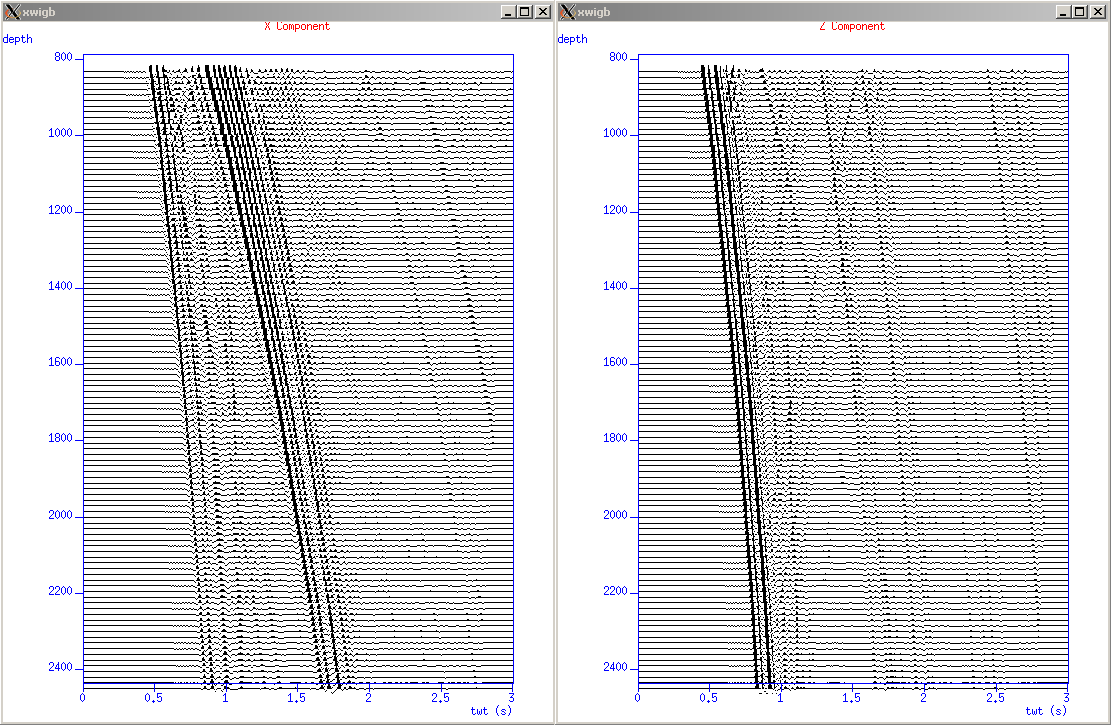
\includegraphics[width=467pt, height=305pt, keepaspectratio=true]{LatihanVSPsu-fig002.png}
%%\caption{This should be the caption for \texttt{LatihanVSPsu-fig002.png}.}
%%\end{figure}

\vspace{16pt}
\begin{center}
\textit{Synthetic Data is usable to identify VSP wave type\pagebreak{}}
\end{center}

\vspace{16pt}
\baselineskip=12pt
\leftskip=0pt
\textbf{Script Source:}

\vspace{4pt}
Filename: CreateElasticSynth.sh

\vspace{4pt}
00001 \#!/bin/bash

\vspace{4pt}
00002 

\vspace{4pt}
00022 \#input

\vspace{4pt}
00023 \#define model dimension

\vspace{4pt}
00024 nx=100

\vspace{4pt}
00025 dx=10

\vspace{4pt}
00026 nz=300

\vspace{4pt}
00027 dz=10

\vspace{4pt}
00028 outputX=HMX.su \#specify filename for horizontal component

\vspace{4pt}
00029 outputZ=Z.su \#specify filename for vertical component

\vspace{4pt}
00030 

\vspace{4pt}
00031 \#set parameter

\vspace{4pt}
00032 \#Ela2D FD setup

\vspace{4pt}
00033 \# * @todo this dt is for FD timestep modeling, should use appropriate 

\vspace{4pt}
dt  for time step modeling

\vspace{4pt}
00034 \# * @todo implement resampling for final su data

\vspace{4pt}
00035 dt=0.002 \#set timestep and will also be samplin rate for out put data, 

\vspace{4pt}
@TODO  CHECK!!

\vspace{4pt}
00036 tmax=3 \#maximum recording time

\vspace{4pt}
00037 f\_cent=30 \#dominant frequency

\vspace{4pt}
00038 

\vspace{4pt}
00039 \#source

\vspace{4pt}
00040 \#setting source, use *.txt from 1BuildFlatModel, convert it to binary 

\vspace{4pt}
for SU header requirement

\vspace{4pt}
00041 \#DO NOT MODIFY LINE AFTER THIS, UNLESS YOU KNOW WHAT YOU ARE DOING

\vspace{4pt}
00042 

\vspace{4pt}
00043 \#copy receiver from 1BuildFlatModel

\vspace{4pt}
00044 cp ../1BuildFlatModel/*.dat .

\vspace{4pt}
00045 cp ../1BuildFlatModel/*.txt .

\vspace{4pt}
00046 

\vspace{4pt}
00047 \#flip receiver list for Ela2D requirement

\vspace{4pt}
00048 awk '\{print \texttt{"}\textbackslash{}t\texttt{"}, \$2, \texttt{"}\textbackslash{}t\texttt{"}, 
\$1\}' receiver\_list.txt \texttt{>} receiver\_list.tmp 

\vspace{4pt}
00049 awk '\{print \texttt{"}\textbackslash{}t\texttt{"}, \$2, \texttt{"}\textbackslash{}t\texttt{"}, 
\$1\}' source\_list.txt \texttt{>} source\_list.tmp

\vspace{4pt}
00050 mv receiver\_list.tmp receiver\_list.txt

\vspace{4pt}
00051 mv source\_list.tmp source\_list.txt

\vspace{4pt}
00052 

\vspace{4pt}
00053 a2b \texttt{<} source\_list.txt \texttt{>} source\_list.bin

\vspace{4pt}
00054 src\_x=(\$(awk '\{print \$1\}' source\_list.txt))

\vspace{4pt}
00055 src\_z=(\$(awk '\{print \$2\}' source\_list.txt))

\vspace{4pt}
00056 \#load receiver

\vspace{4pt}
00057 a2b \texttt{<} receiver\_list.txt \texttt{>} receiver\_list.bin

\vspace{4pt}
00058 nrec=(\$(wc -l receiver\_list.txt \textbar{} awk '\{print \$1\}'))

\vspace{4pt}
00059 ns=(\$(echo \$tmax/\$dt+1 \textbar{}bc -l))

\vspace{4pt}
00060 

\vspace{4pt}
00061 \#substitute all input variables to Ela2D param \& in file

\vspace{4pt}
00062 sed -e \texttt{"}s/src\_x/\$src\_x/\texttt{"} -e \texttt{"}s/src\_z/\$src\_z/\texttt{"} 
\textbackslash{}

\vspace{4pt}
00063 -e \texttt{"}s/seddt/\$dt/\texttt{"} -e \texttt{"}s/sedtmax/\$tmax/\texttt{"} 
-e \texttt{"}s/sedf\_cent/\$f\_cent/\texttt{"} \textbackslash{}

\vspace{4pt}
00064 -e \texttt{"}s/nrec/\$nrec/\texttt{"} \textbackslash{}

\vspace{4pt}
00065  \texttt{<} ./template/ela2d.in.template \texttt{>} ela2d.in.tmp

\vspace{4pt}
00066 

\vspace{4pt}
00067 sed -e \texttt{"}s/seddx/\$dx/\texttt{"} -e \texttt{"}s/seddz/\$dz/\texttt{"} 
\textbackslash{}

\vspace{4pt}
00068 -e \texttt{"}s/sednx/\$nx/\texttt{"} -e \texttt{"}s/sednz/\$nz/\texttt{"} 
\textbackslash{}

\vspace{4pt}
00069  \texttt{<} ./template/grid.param.template \texttt{>} grid.param

\vspace{4pt}
00070  

\vspace{4pt}
00071 cat ela2d.in.tmp receiver\_list.txt \texttt{>} ela2d.in

\vspace{4pt}
00072 

\vspace{4pt}
00073 \#Running Ela2D

\vspace{4pt}
00074 echo \texttt{"}Start Ela2D\texttt{"}

\vspace{4pt}
00075 ela2d

\vspace{4pt}
00076 

\vspace{4pt}
00077 echo \texttt{"}Convert Ela2D output to SU Format\texttt{"}

\vspace{4pt}
00078 dtms=(\$(echo \$dt*1000000 \textbar{}bc -l))

\vspace{4pt}
00079 suaddhead \texttt{<} seismicX.H@ ns=\$ns \textbar{}

\vspace{4pt}
00080 sushw key=dt a=\$dtms \textbar{}

\vspace{4pt}
00081 sushw key=gx,gelev infile=receiver\_list.bin \textbar{}

\vspace{4pt}
00082 sushw key=sx a=\$src\_x b=0 j=\$nrec \textbar{}

\vspace{4pt}
00083 sushw key=selev a=\$src\_z b=0 j=\$nrec \texttt{>} \$outputX

\vspace{4pt}
00084 

\vspace{4pt}
00085 suaddhead \texttt{<} seismicZ.H@ ns=\$ns \textbar{}

\vspace{4pt}
00086 sushw key=dt a=\$dtms \textbar{}

\vspace{4pt}
00087 sushw key=gx,gelev infile=receiver\_list.bin \textbar{}

\vspace{4pt}
00088 sushw key=sx a=\$src\_x b=0 j=\$nrec  \textbar{}

\vspace{4pt}
00089 sushw key=selev a=\$src\_z b=0 j=\$nrec \texttt{>} \$outputZ

\vspace{4pt}
00090 

\vspace{4pt}
00091 \#clean Up

\vspace{4pt}
00092 mv *.H* *.out ela2d\_dir 

\vspace{4pt}
00093 rm *.tmp *.bin 

\vspace{4pt}
00094 echo \texttt{"}Ela2D Finished\texttt{"}

\vspace{4pt}
00095 

\vspace{4pt}
00096 \#display

\vspace{4pt}
00097 suxwigb \texttt{<} \$outputX title=\texttt{"}X Component\texttt{"} perc=97 
style=vsp key=gelev 

\vspace{4pt}
\parindent=18pt
label2=\texttt{"}depth\texttt{"} label1=\texttt{"}twt (s)\texttt{"} \&

\vspace{4pt}
\parindent=0pt
00098 suxwigb \texttt{<} \$outputZ title=\texttt{"}Z Component\texttt{"} perc=97 
style=vsp key=gelev 

\vspace{4pt}
\parindent=18pt
label2=\texttt{"}depth\texttt{"} label1=\texttt{"}twt (s)\texttt{"} \&

\vspace{4pt}
\parindent=0pt
00099 \pagebreak{}

\vspace{24pt}
\subsection*{{\large{}\textbf{3BreakTimePick/FBAutoPick.sh File Reference}}}

\vspace{12pt}
23BreakTimePick/FBAutoPick.sh3BreakTimePick/FBAutoPick.sh\label{AAAAAAAAAI}

\vspace{12pt}
Automatic FB picking. 

\vspace{24pt}
\subsubsection*{\textbf{Detailed Description}}

\vspace{1pt}
Break time picking is the most crucial for every VSP job. Every VSP analysis is 
based and required break time pick. SU provides good tools but not yet sophisticated 
and user friendly to do manual break time pick. The script for manual picking using 
ximage and button [s] functionality is \textit{\textbf{BreakTimePick.sh.}} 

\vspace{1pt}
We are going to use automatic break time picking from SU, and smooth it a little 
bit using octave script. A QC of breaktime picking, besides visual QC, is to compute 
interval velocity and compare it with sonic lo velocity; this will be done on DisplayPicks.sh.

\vspace{1pt}
The feature of transit time correction to seismic reference datum (SRD) through 
cosine correction has not been implemented.

\vspace{4pt}
\textbf{Usage:}

\vspace{4pt}
Open the file in text editor, and edit required parameters as necessary. The parameter 
description is given here. Run the command from console. 

\vspace{16pt}
\$./CreateElasticSynthetic.sh 

\vspace{16pt}
*** Before running the script, please manually copy the SU file that you want to 
pick to this directory , for example:

\vspace{4pt}
\$cp ../2Ela2D/Z.su 

\vspace{4pt}
.

\vspace{4pt}
\textbf{Output:}

\vspace{4pt}
- SU File after automatic picking, the breaktime pick saved in \textit{unscale 
}header

\vspace{4pt}
- ASCII File containing Transit Time picking (format: [Transit Time][Depth]

\vspace{4pt}
\textbf{Parameters:}

\vspace{4pt}
\textit{input} SU file to be picked 

\vspace{4pt}
\begin{tabular}{|>{\raggedright}p{54pt}|>{\raggedright}p{245pt}|}
\hline
\tabularnewline
\hline
o\textit{utput}  & SU file after picked \tabularnewline
\hline
o\textit{utput\_picks}  & ASCII file for automatic Transit Time pick result \tabularnewline
\hline
\end{tabular}

\vspace{1pt}
Definition in file \textbf{FBAutoPick.sh}.

\vspace{4pt}
\textbf{Author:}

\vspace{4pt}
\leftskip=18pt
fahdi@gm2001.net 

\vspace{4pt}
\leftskip=0pt
\textbf{Date:}

\vspace{4pt}
\leftskip=18pt
February 2012 

\vspace{16pt}
\leftskip=0pt
\textbf{Output Example:\pagebreak{}}

\vspace{4pt}
\$./DisplayPicks.sh

\vspace{4pt}
\begin{center}
%%\begin{figure}[htbp]
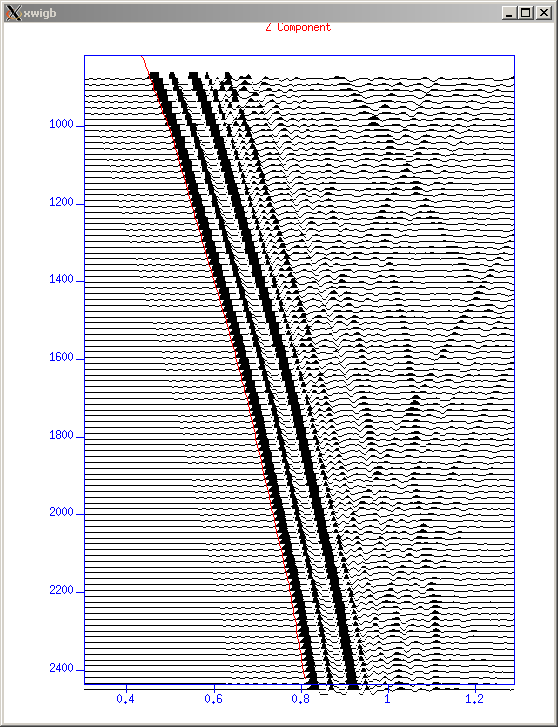
\includegraphics[width=239pt, height=311pt, keepaspectratio=true]{LatihanVSPsu-fig003.png}
%%\caption{This should be the caption for \texttt{LatihanVSPsu-fig003.png}.}
%%\end{figure}

\vspace{16pt}
\textit{Breaktime pick displayed with red curve}

\vspace{16pt}
%%\begin{figure}[htbp]
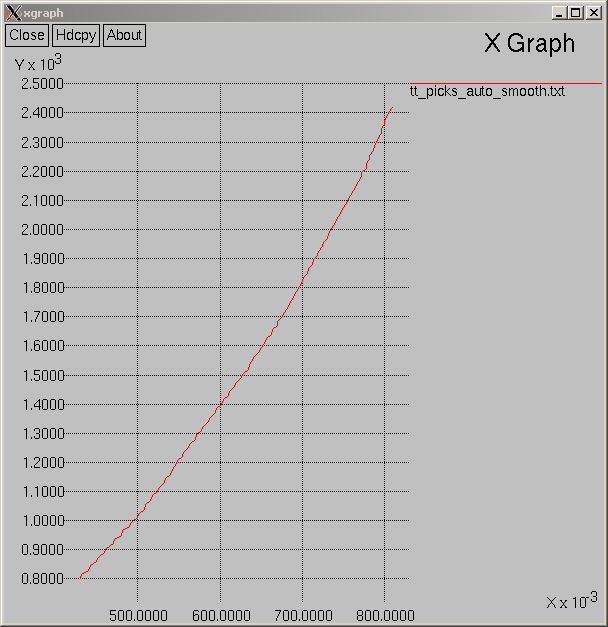
\includegraphics[width=237pt, height=245pt, keepaspectratio=true]{LatihanVSPsu-fig004.png}
%%\caption{This should be the caption for \texttt{LatihanVSPsu-fig004.png}.}
%%\end{figure}

\vspace{16pt}
\textit{Time-Depth Curve\pagebreak{}}
\end{center}

\vspace{4pt}
\baselineskip=12pt
\leftskip=0pt
\textbf{Script Source:}

\vspace{4pt}
Filename: FBAutoPick.sh

\vspace{16pt}
00001 \#!/bin/bash

\vspace{4pt}
00002 \label{l00014}

\vspace{4pt}
00014 \#input

\vspace{4pt}
00015 input=Z.su

\vspace{4pt}
00016 output=Z\_picked.su \#breaktime will saved at unscale header in this file

\vspace{4pt}
00017 output\_picks=tt\_picks\_auto.txt \#ASCII output of breaktime picking 

\vspace{4pt}
00018 

\vspace{4pt}
00019 \#process

\vspace{4pt}
00020 \#do automatic picking

\vspace{4pt}
00021 sufbpickw \texttt{<} \$input \texttt{>} \$output

\vspace{4pt}
00022 \#a little housekeeping 

\vspace{4pt}
00023 sugethw \texttt{<} \$output key=unscale,gelev \textbar{} sed -e 's/unscale=//' 
-e 

\vspace{4pt}
's/gelev=//'\textbar{} sed '/\textasciicircum{}\$/d' \textbar{} sort -bn -k 2 \textbar{} 
uniq \texttt{>} \$output\_picks

\vspace{4pt}
00024 nrec=(\$(wc -l tt\_picks\_auto.txt \textbar{} awk '\{print \$1\}')) \#calculate 
number 

\vspace{4pt}
of receiver

\vspace{4pt}
00025 

\vspace{4pt}
00026 \#display data and picks

\vspace{4pt}
00027 suxwigb \texttt{<} \$input title=\texttt{"}Z Component\texttt{"} perc=97 
style=vsp key=gelev 

\vspace{4pt}
\parindent=18pt
curve=\$output\_picks npair=\$nrec,1 curvecolor=red label2=\texttt{"}depth\texttt{"} 

\vspace{4pt}
label1=\texttt{"}twt (s)\texttt{"}\&

\vspace{4pt}
\parindent=0pt
00028 

\vspace{4pt}
00029 \#smoothing

\vspace{4pt}
00030 octave --silent --eval \texttt{"}ttSmoothing('\$output\_picks')\texttt{"};

\vspace{4pt}
00031 

\vspace{4pt}
00032 \#clean up

\vspace{4pt}
00033 rm test.su

\vspace{4pt}
00034 

\vspace{4pt}
00035 

\vspace{4pt}
00036 \newpage

\newpage
\vspace{12pt}
\subsection*{{\large{}\textbf{4Preprocessing/FrequencyAnalysis.sh File Reference}}}

\vspace{12pt}
24Preprocessing/FrequencyAnalysis.sh4Preprocessing/FrequencyAnalysis.sh\label{AAAAAAAAAJ}

\vspace{12pt}
Create FZ Spectrum \& FK-Spectrum. 

\vspace{24pt}
\subsubsection*{\textbf{Detailed Description}}

\vspace{1pt}
Analysis of frequency content in VSP is also significant process. If we compute 
frequency spectrum of each traces, we are going to have frequency profile each 
depth. These profiles will also describing quality factor/attenuation. FK Spectrum 
is also important to see how far the aliasing is.

\vspace{4pt}
\textbf{Usage:}

\vspace{4pt}
Open the file in text editor, and edit required parameters as necessary. The parameter 
description is given here. Run the command from console. 

\vspace{16pt}
\$./FrequencyAnalysis.sh 

\vspace{16pt}
*** Before running the script, please manually copy the SU file that you want to 
pick to this directory , for example:

\vspace{4pt}
\$cp ../0ImportSEGY/realZ.su .

\vspace{4pt}
\$cp ../0ImportSEGY/tt-header.txt .

\vspace{16pt}
\textbf{Output:}

\vspace{4pt}
- SU File for Frequency vs Depth \& Frequency vs Wavenumber

\vspace{16pt}
\textbf{Parameters:}

\vspace{4pt}
\textit{input} SU file to analyze 

\vspace{4pt}
\begin{tabular}{|>{\raggedright}p{54pt}|>{\raggedright}p{245pt}|}
\hline
\tabularnewline
\hline
o\textit{utput\_fz}  & Spectrum of Frequency vs Depth in SU format \tabularnewline
\hline
o\textit{utput\_fk}  & Spectrum of Frequency vs Wavenumber in SU format \tabularnewline
\hline
\end{tabular}

\vspace{1pt}
Definition in file \textbf{FrequencyAnalysis.sh}.

\vspace{4pt}
\textbf{Author:}

\vspace{4pt}
\leftskip=18pt
fahdi@gm2001.net 

\vspace{4pt}
\leftskip=0pt
\textbf{Date:}

\vspace{4pt}
\leftskip=18pt
February 2012 

\vspace{16pt}
\leftskip=0pt
\textbf{Output Example:\pagebreak{}}

\vspace{4pt}
\$./FrequencyAnalysis.sh

\vspace{28pt}
%%\begin{figure}[htbp]
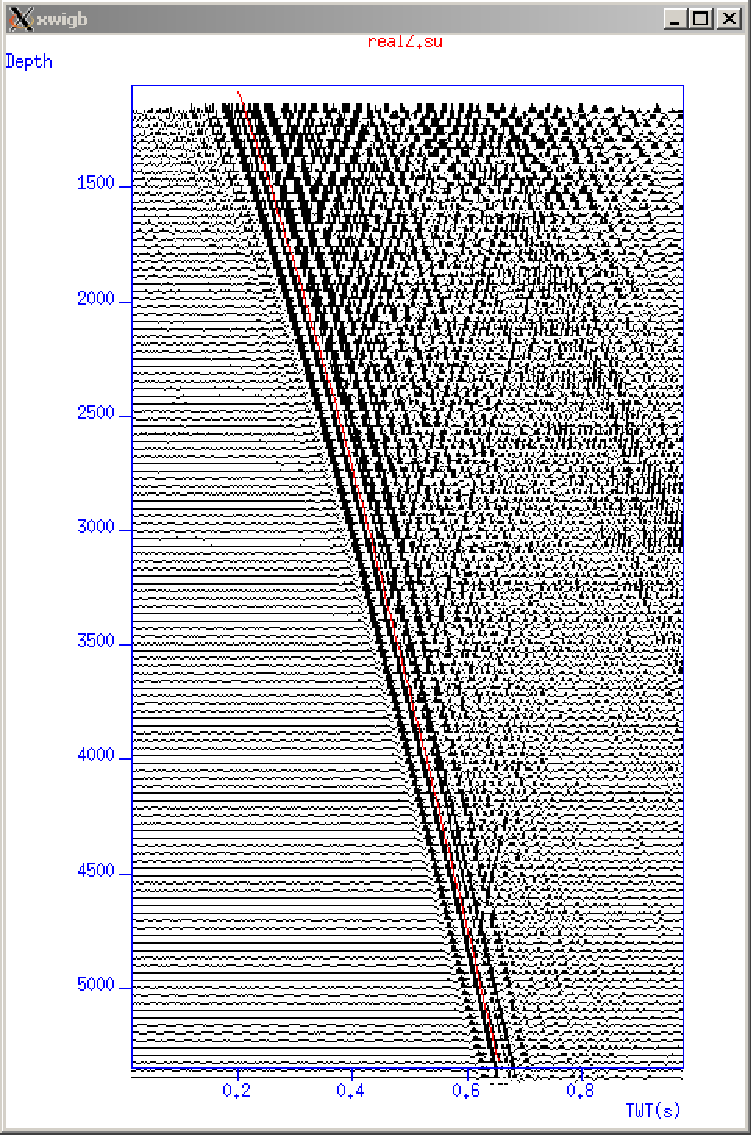
\includegraphics[width=166pt, height=251pt, keepaspectratio=true]{LatihanVSPsu-fig005.pdf}
%%\caption{This should be the caption for \texttt{LatihanVSPsu-fig005.pdf}.}
%%\end{figure}

\vspace{280pt}
\begin{center}
\textit{Real Data- Note The break time on red curve. }

\vspace{16pt}
%%\begin{figure}[htbp]
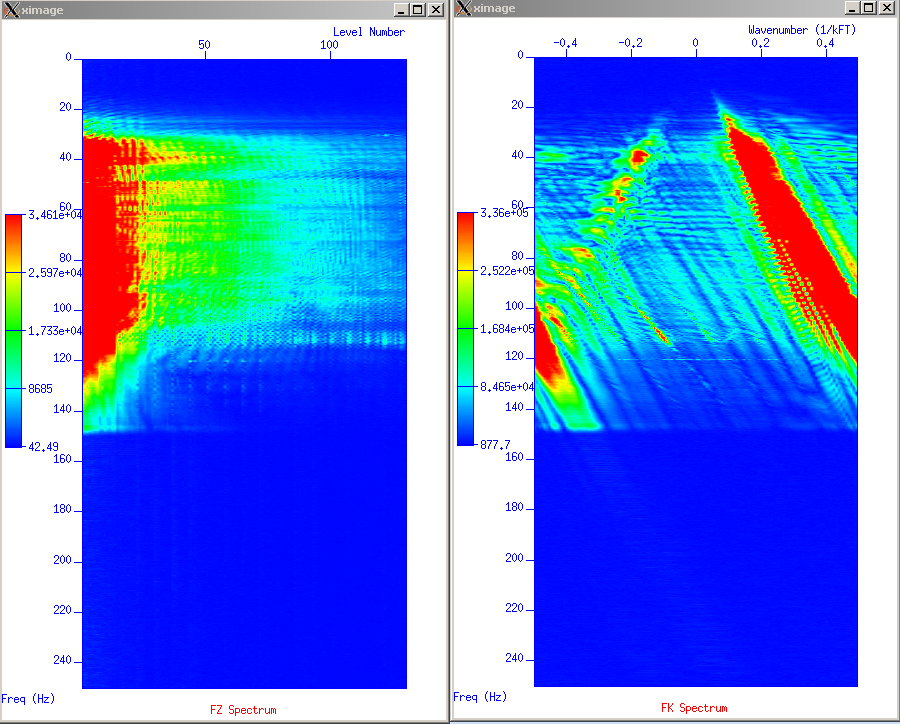
\includegraphics[width=351pt, height=282pt, keepaspectratio=true]{LatihanVSPsu-fig006.png}
%%\caption{This should be the caption for \texttt{LatihanVSPsu-fig006.png}.}
%%\end{figure}

\vspace{16pt}
\textit{The FZ and FK Spectrum\pagebreak{}}
\end{center}

\vspace{16pt}
\baselineskip=12pt
\leftskip=0pt
\textbf{Script Source:}

\vspace{4pt}
Filename: FBAutoPick.sh

\vspace{16pt}
00001 \#!/bin/bash

\vspace{4pt}
00002 

\vspace{4pt}
00014 \#input

\vspace{4pt}
00015 input=realZ.su

\vspace{4pt}
00016 output\_fz=z-spec-fz.su

\vspace{4pt}
00017 output\_fk=z-spec-fk.su

\vspace{4pt}
00018 

\vspace{4pt}
00019 \#compute fz

\vspace{4pt}
00020 suspecfx \texttt{<} \$input \texttt{>} \$output\_fz

\vspace{4pt}
00021 

\vspace{4pt}
00022 \#compute fk

\vspace{4pt}
00023 suspecfk \texttt{<} \$input \texttt{>} \$output\_fk

\vspace{4pt}
00024 

\vspace{4pt}
00025 \#display

\vspace{4pt}
00026 nrec=(\$(wc -l tt-header.txt \textbar{} awk '\{print \$1\}'))

\vspace{4pt}
00027 suxwigb \texttt{<} \$input title=\$input perc=97 style=vsp key=gelev 

\vspace{4pt}
\parindent=18pt
curve=tt-header.txt npair=\$nrec,1 curvecolor=red label2=\texttt{"}Depth\texttt{"} 

\vspace{4pt}
label1=\texttt{"}TWT(s)\texttt{"}\&

\vspace{4pt}
\parindent=0pt
00028 

\vspace{4pt}
00029 \#displayfz

\vspace{4pt}
00030 suximage \texttt{<} \$output\_fz cmap=hsv2 perc=95 legend=1 title='FZ Spectrum' 

\vspace{4pt}
\parindent=18pt
label1='Freq (Hz)' label2='Level Number' \&

\vspace{4pt}
\parindent=0pt
00031 

\vspace{4pt}
00032 \#displayfk

\vspace{4pt}
00033 suximage \texttt{<} \$output\_fk cmap=hsv2 perc=95 legend=1 title='FK Spectrum' 

\vspace{4pt}
\parindent=18pt
label1='Freq (Hz)' label2='Wavenumber (1/kFT)' \& 

\vspace{4pt}
\parindent=0pt
00034 

\vspace{4pt}
00035 \newpage

\newpage
\vspace{12pt}
\subsection*{{\large{}\textbf{4Preprocessing/Preprocessing.sh File Reference}}}

\vspace{12pt}
24Preprocessing/Preprocessing.sh4Preprocessing/Preprocessing.sh\label{AAAAAAAAAK}

\vspace{12pt}
Do Preprocessing: BPF, Normalize, TVG. 

\vspace{24pt}
\subsubsection*{\textbf{Detailed Description}}

\vspace{1pt}
This step is to perform preprocessing before we process VSP signal.

\vspace{1pt}
The BPF is required to eliminate noise based on their frequency content. The frequency 
of data needs to be analyzed first; you can use FrequencyAnalysis.sh script to 
do this

\vspace{1pt}
For some VSP tools, the coupling between tools and formation is not the same, and 
sometimes there is energy variation between shot to shot, which makes median filter 
not working properly. This is compensated by statistically normalize the data based 
on downgoing event. SU does not have the capability to do RMS calculation based 
on isolated downgoing event (say analyze for 200 ms after first break), but using 
sugain to normalize the data should be enough for this exercise. 

\vspace{1pt}
The Time Varying Gain/Exponential Gain is required to correct the spherical divergence 
effect.

\vspace{1pt}
Workflow that has been set on Preprocessing.sh is just based on personal experience; 
you can modify it as necessary. The workflow is BPF + RMS Normalization + TimeVaryingGain

\vspace{4pt}
\textbf{Usage:}

\vspace{4pt}
Open the file in text editor, and edit required parameters as necessary. The parameter 
description is given here. Run the command from console. 

\vspace{4pt}
\$./Preprocessing.sh 

\vspace{16pt}
*** Before running the script, please manually copy the SU file that you want to 
pick to this directory , for example:

\vspace{4pt}
\$cp ../0ImportSEGY/realZ.su

\vspace{16pt}
\textbf{Output:}

\vspace{4pt}
- SU file for each process (after BPF, after BPF+Normalization, after BPF+Normalization+TimeVaryingGain

\vspace{4pt}
- Final SU after preprocessing with proper filenaming 

\vspace{4pt}
\textbf{Parameters:}

\vspace{4pt}
\textit{input} SU file to process 

\vspace{4pt}
\begin{tabular}{|>{\raggedright}p{54pt}|>{\raggedright}p{245pt}|}
\hline
\tabularnewline
\hline
o\textit{utput\_bpf}  & output SU file after BPF filter \tabularnewline
\hline
b\textit{pf}  & Four points of BPF filter \tabularnewline
\hline
o\textit{utput\_norm}  & output SU file after normalization (RMS whole window operation) 
\tabularnewline
\hline
o\textit{utput\_tvg}  & SU file after TimeVaryingGain ( \tabularnewline
\hline
t\textit{pow}  & TVG constant \tabularnewline
\hline
f\textit{inal\_output}  & Output after all preprocessing workflow in SU format 
\tabularnewline
\hline
\end{tabular}

\vspace{1pt}
Definition in file \textbf{Preprocessing.sh}.

\vspace{4pt}
\textbf{Author:}

\vspace{4pt}
\leftskip=18pt
fahdi@gm2001.net 

\vspace{4pt}
\leftskip=0pt
\textbf{Date:}

\vspace{4pt}
\leftskip=18pt
February 2012 

\vspace{40pt}
\leftskip=0pt
\textbf{Output Example:}

\vspace{4pt}
\$./Preprocessing.sh

\vspace{16pt}
\begin{center}
%%\begin{figure}[htbp]
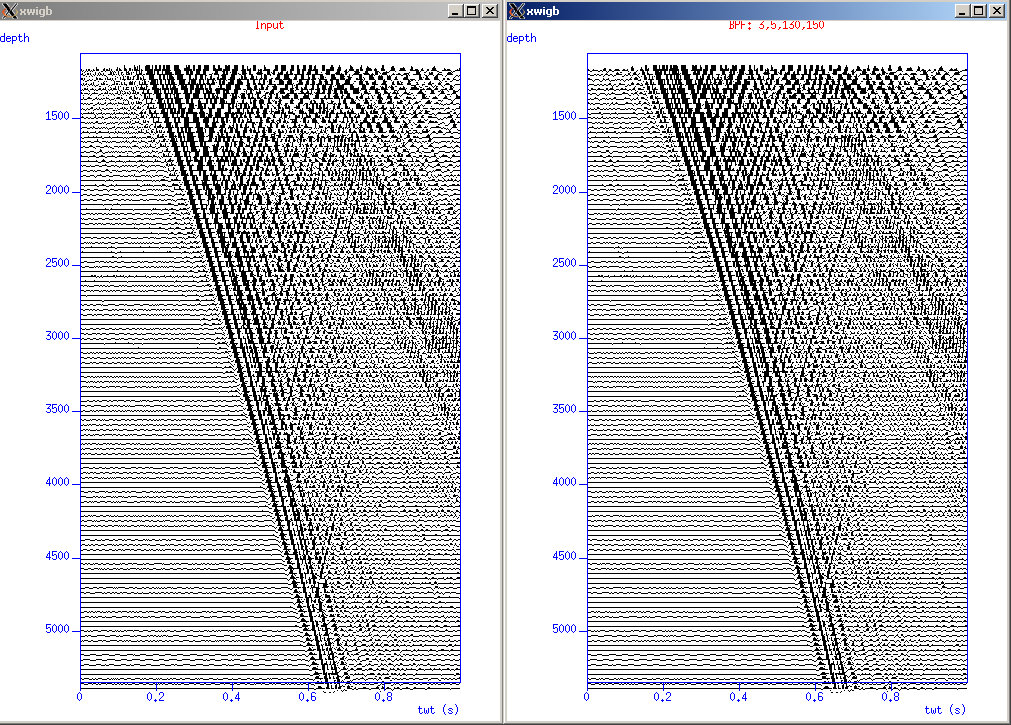
\includegraphics[width=372pt, height=261pt, keepaspectratio=true]{LatihanVSPsu-fig007.png}
%%\caption{This should be the caption for \texttt{LatihanVSPsu-fig007.png}.}
%%\end{figure}

\vspace{16pt}
\textit{Input (left), Input after BPF (right)}

\vspace{16pt}
%%\begin{figure}[htbp]
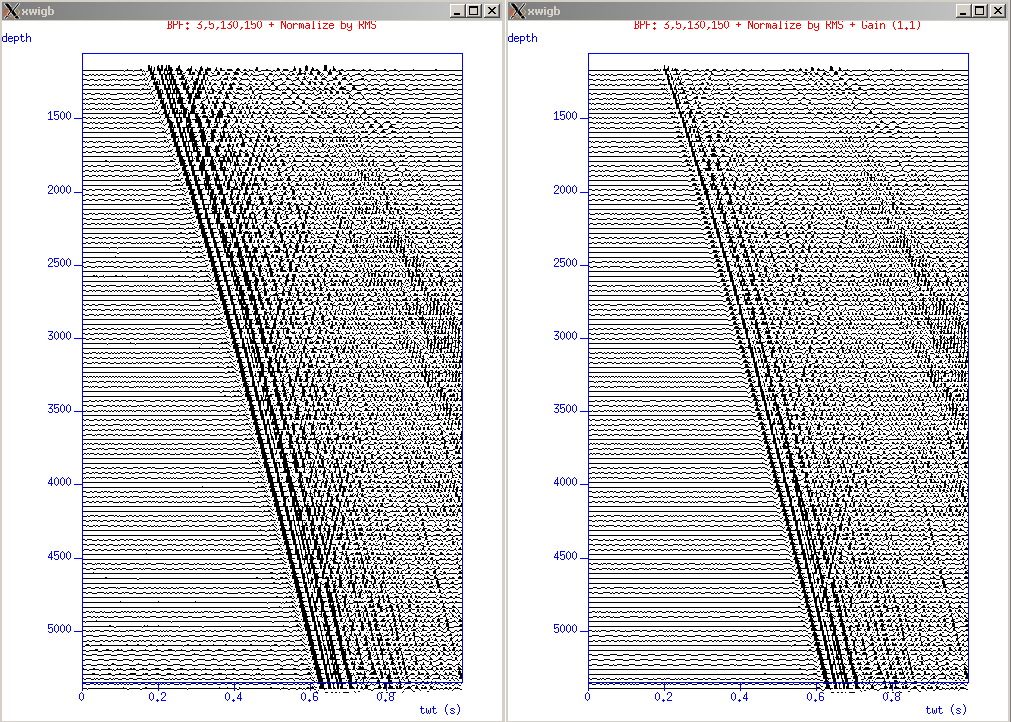
\includegraphics[width=364pt, height=260pt, keepaspectratio=true]{LatihanVSPsu-fig008.png}
%%\caption{This should be the caption for \texttt{LatihanVSPsu-fig008.png}.}
%%\end{figure}

\vspace{16pt}
\textit{Input after BPF+Normalize (left) Input after BPF+Normalize+TimeVaryingGain 
(right)}
\end{center}

\vspace{40pt}
\baselineskip=12pt
\leftskip=0pt
\textbf{Script Source:}

\vspace{4pt}
Filename: Preprocessing.sh

\vspace{16pt}
00001 \#!/bin/bash

\vspace{4pt}
00002 

\vspace{4pt}
00018 \#input

\vspace{4pt}
00019 input=realZ.su

\vspace{4pt}
00020 output\_bpf=Z\_picked\_bpf.su \# output after BPF

\vspace{4pt}
00021 output\_norm=Z\_picked\_bpf\_norm.su \#output after BPF followed RMS 

\vspace{4pt}
Normalization

\vspace{4pt}
00022 output\_tvg=Z\_picked\_bpf\_norm\_tvg.su \#output after BPF followed RMS 

\vspace{4pt}
Normalization followed by TimeVaryingGain

\vspace{4pt}
00023 final\_output=Z\_prepro.su \#housekeeping to make naming convention

\vspace{4pt}
00024 

\vspace{4pt}
00025 \#set parameter

\vspace{4pt}
00026 bpf=3,5,130,150 \#4 points bandpass specification

\vspace{4pt}
00027 tpow=1.1 \#multiply data by t\textasciicircum{}tpow

\vspace{4pt}
00028 

\vspace{4pt}
00029 \#bpf

\vspace{4pt}
00030 sufilter \texttt{<} \$input f=\$bpf \texttt{>} \$output\_bpf

\vspace{4pt}
00031 

\vspace{4pt}
00032 \#normalize by dividing with RMS

\vspace{4pt}
00033 sugain \texttt{<} \$output\_bpf pbal=1 \texttt{>} \$output\_norm

\vspace{4pt}
00034 

\vspace{4pt}
00035 \#run exponential gain

\vspace{4pt}
00036 sugain \texttt{<} \$output\_norm tpow=\$tpow \texttt{>} \$output\_tvg

\vspace{4pt}
00037 cp \$output\_tvg \$final\_output \#housekeeping to make naming convention

\vspace{4pt}
00038 

\vspace{4pt}
00039 \#display

\vspace{4pt}
00040 suxwigb \texttt{<} \$input title=\texttt{"}Input\texttt{"} perc=97 style=vsp 
key=gelev 

\vspace{4pt}
label2=\texttt{"}depth\texttt{"} label1=\texttt{"}twt (s)\texttt{"} x1beg=0.0 x1end=1.0 
xbox=10 wbox=500\&

\vspace{4pt}
00041 suxwigb \texttt{<} \$output\_bpf title=\texttt{"}BPF: \$bpf\texttt{"} perc=97 
style=vsp key=gelev 

\vspace{4pt}
label2=\texttt{"}depth\texttt{"} label1=\texttt{"}twt (s)\texttt{"} x1beg=0.0 x1end=1.0 
xbox=520 wbox=500\&

\vspace{4pt}
00042 suxwigb \texttt{<} \$output\_norm title=\texttt{"}BPF: \$bpf + Normalize 
by RMS\texttt{"} perc=97 

\vspace{4pt}
style=vsp key=gelev label2=\texttt{"}depth\texttt{"} label1=\texttt{"}twt (s)\texttt{"} 
x1beg=0.0 

\vspace{4pt}
x1end=1.0 xbox=10 wbox=500\&

\vspace{4pt}
00043 suxwigb \texttt{<} \$output\_tvg title=\texttt{"}BPF: \$bpf + Normalize by 
RMS + Gain 

\vspace{4pt}
(\$tpow)\texttt{"} perc=97 style=vsp key=gelev label2=\texttt{"}depth\texttt{"} 
label1=\texttt{"}twt (s)\texttt{"} 

\vspace{4pt}
x1beg=0.0 x1end=1.0 xbox=520 wbox=500\&\newpage

\newpage
\vspace{24pt}
\subsection*{{\large{}\textbf{5Separation/Separation.sh File Reference}}}

\vspace{12pt}
25Separation/Separation.sh5Separation/Separation.sh\label{AAAAAAAAAM}

\vspace{12pt}
Run wavefield separation based on TT using median velocity filter. 

\vspace{24pt}
\subsubsection*{\textbf{Detailed Description}}

\vspace{1pt}
Wavefield separation is another crucial step in VSP processing. The process is 
to get the upgoing (reflection wave) from the total wavefield. As we have seen 
between downgoing and upgoing can be differentiate clearly by their slope, downgoing 
is positive towards depth, and upgoing is negative. Based on these two different 
slopes, we can separate this using velocity filter (slope \textasciitilde{} velocity), 
by aligning them along the slopes. After alignment, the signal that has same slopes 
will be coherent, and using median filter, you can get coherent signal, and the 
uncoherent signal will be the residual signal (subtracted from total signal). 

\vspace{1pt}
For example, to extract downgoing, you will align the data by subracting using 
TT, the downgoing will be coherent along the TT, and you can run median filter 
to extract this downgoing. The uncoherent signal will be the residual. 

\vspace{1pt}
Normally the workflow is you extract downgoing first, and subtract this downgoing 
from the total wavefield. You will get residual wavefield (residual1 = total-downgoing). 
And you run second velocity filter, to extract upgoing by aligning to the upgoing 
slope, the input for this is the residual wavefield. 

\vspace{1pt}
Input for separation is normally wavefield after preprocessing.

\vspace{4pt}
\textbf{Usage:}

\vspace{4pt}
Open the file in text editor, and edit required parameters as necessary. The parameter 
description is given here. Run the command from console. 

\vspace{4pt}
\$./Separation.sh 

\vspace{16pt}
*** Before running the script, please manually copy the SU file that you want to 
pick to this directory , for example:

\vspace{4pt}
\$cp ../4Preprocessing/Z\_prepro.su .

\vspace{4pt}
\$cp ../3BreakTimePick/tt-header.txt .

\vspace{16pt}
\textbf{Output:}

\vspace{4pt}
- SU file for each process (downgoing wavefield, residual after downgoing removal, 
upgoing wavefield, residual after after upgoing wavefield extraction

\vspace{16pt}
\textbf{Parameters:}

\vspace{4pt}
\textit{input} SU file to separate after PreProcessing 

\vspace{4pt}
\begin{tabular}{|>{\raggedright}p{54pt}|>{\raggedright}p{245pt}|}
\hline
\tabularnewline
\hline
o\textit{utput\_dn}  & Downgoing wavefield \tabularnewline
\hline
o\textit{utput\_res}  & Residual Wavefield after downgoing wavefield subtraction 
\tabularnewline
\hline
o\textit{utput\_up}  & Upgoing wavefield (Enhanced Residual) \tabularnewline
\hline
o\textit{utput\_res2}  & 2nd Residual after Upgoing extraction \tabularnewline
\hline
t\textit{imePicks}  & ASCII file containing transit time picking \tabularnewline
\hline
l\textit{evel\_down}  & number median level for downngoing extraction \tabularnewline
\hline
l\textit{evel\_up}  & number median level for upgoing extraction \tabularnewline
\hline
\end{tabular}

\vspace{1pt}
Definition in file \textbf{Separation.sh}.

\vspace{4pt}
\textbf{Author:}

\vspace{4pt}
\leftskip=18pt
fahdi@gm2001.net 

\vspace{4pt}
\leftskip=0pt
\textbf{Date:}

\vspace{4pt}
\leftskip=18pt
February 2012 

\vspace{16pt}
\leftskip=0pt
\textbf{Output Example:}

\vspace{4pt}
\$./Separation.sh\&

\vspace{4pt}
\$./DisplaySeparation.sh \&

\vspace{16pt}
\begin{center}
%%\begin{figure}[htbp]
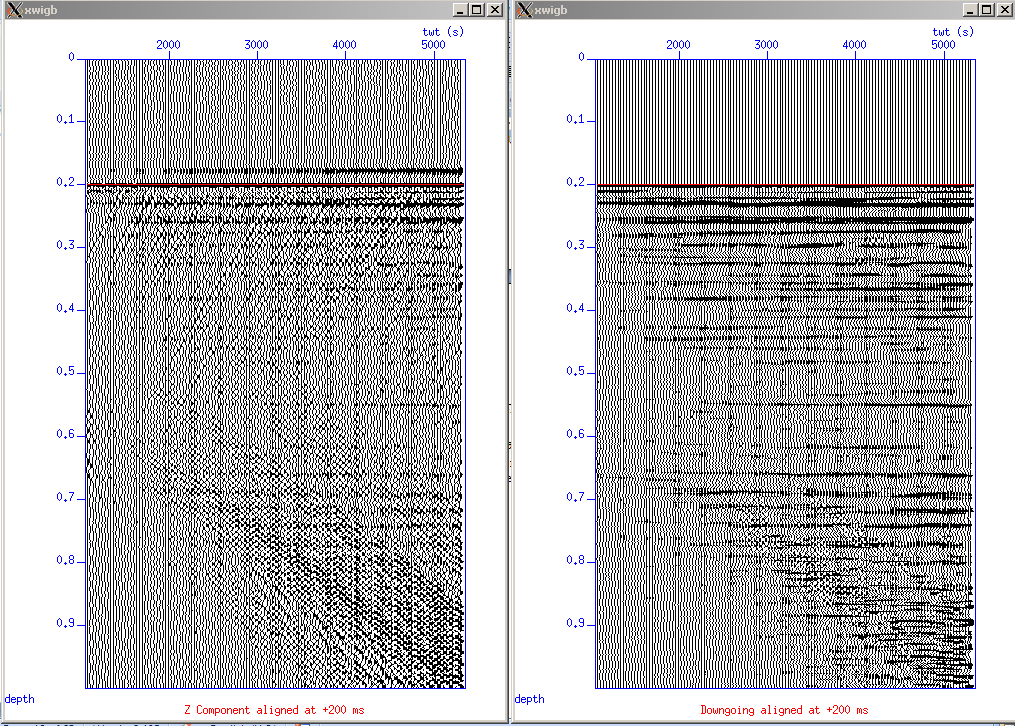
\includegraphics[width=343pt, height=245pt, keepaspectratio=true]{LatihanVSPsu-fig009.png}
%%\caption{This should be the caption for \texttt{LatihanVSPsu-fig009.png}.}
%%\end{figure}

\vspace{16pt}
\textit{Z component total wavefield aligned at -TT (left) and Downgoing Wavefield 
(right)}

\vspace{16pt}
%%\begin{figure}[htbp]
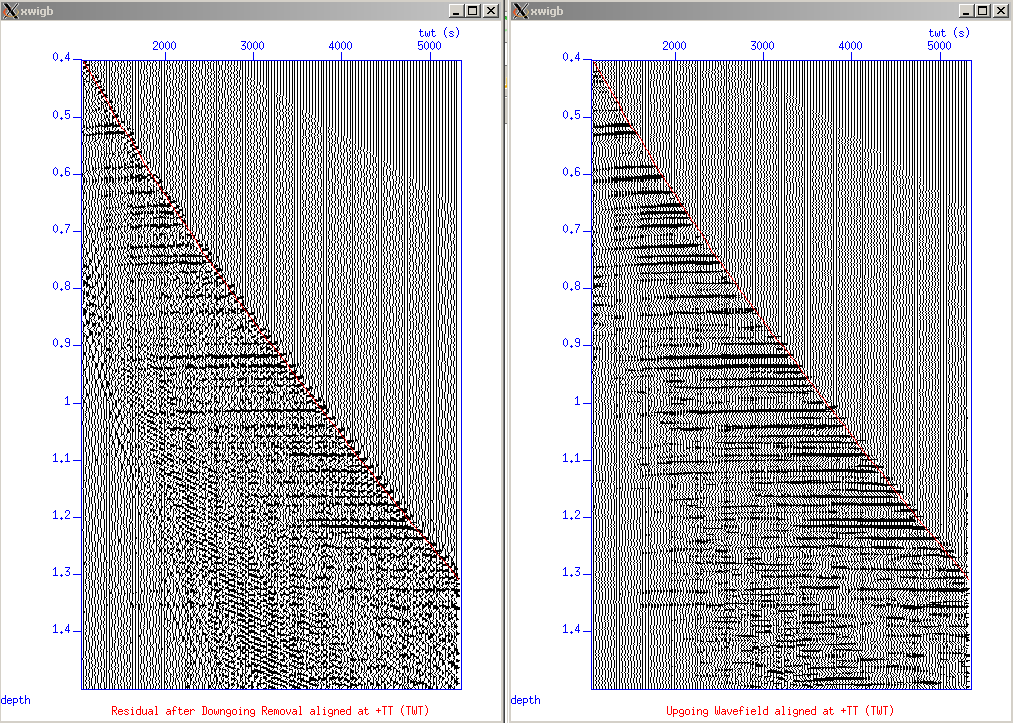
\includegraphics[width=334pt, height=239pt, keepaspectratio=true]{LatihanVSPsu-fig010.png}
%%\caption{This should be the caption for \texttt{LatihanVSPsu-fig010.png}.}
%%\end{figure}

\vspace{16pt}
\textit{Residual wavefield after downgoing wavefield removal aligned at twt (left) 
upgoing wavefield aligned at twt (right)\pagebreak{}}
\end{center}

\vspace{4pt}
\baselineskip=12pt
\leftskip=0pt
\textbf{Script Source:}

\vspace{4pt}
Filename: Separation.sh

\vspace{16pt}
00001 \#!/bin/bash

\vspace{4pt}
00002 

\vspace{4pt}
00018 \#input

\vspace{4pt}
00019 input=Z\_prepro.su

\vspace{4pt}
00020 output\_dn=velf\_dn.su

\vspace{4pt}
00021 output\_res=velf\_res.su

\vspace{4pt}
00022 output\_up=velf\_up.su

\vspace{4pt}
00023 output\_res2=velf\_res2.su

\vspace{4pt}
00024 timePicks=tt-header.txt

\vspace{4pt}
00025 

\vspace{4pt}
00026 \#set parameter

\vspace{4pt}
00027 level\_down=9

\vspace{4pt}
00028 level\_up=7

\vspace{4pt}
00029 

\vspace{4pt}
00030 

\vspace{4pt}
00031 \#housekeeping

\vspace{4pt}
00032 nrec=(\$(wc -l \$timePicks \textbar{} awk '\{print \$1\}')) \#housekeeping, 
check 

\vspace{4pt}
number of receiver

\vspace{4pt}
00033 

\vspace{4pt}
00034 awk '\{print \$2\}' \$timePicks \texttt{>} xfile.tmp

\vspace{4pt}
00035 a2b \texttt{<} xfile.tmp n1=\$nrec\texttt{>} xfile.bin

\vspace{4pt}
00036 

\vspace{4pt}
00037 awk '\{print \$1\}' \$timePicks \texttt{>} tfile.tmp

\vspace{4pt}
00038 a2b \texttt{<} tfile.tmp n1=\$nrec\texttt{>} tfile.bin

\vspace{4pt}
00039 

\vspace{4pt}
00040 \#processing

\vspace{4pt}
00041 

\vspace{4pt}
00042 sumedian \texttt{<} \$input xfile=xfile.bin tfile=tfile.bin key=gelev 

\vspace{4pt}
nshift=\$nrec subtract=0 median=1 nmed=\$level\_down sign=-1\texttt{>} \$output\_dn

\vspace{4pt}
00043 sumedian \texttt{<} \$input xfile=xfile.bin tfile=tfile.bin key=gelev 

\vspace{4pt}
nshift=\$nrec subtract=1 median=1 nmed=\$level\_down sign=-1\texttt{>} \$output\_res

\vspace{4pt}
00044 sumedian \texttt{<} \$output\_res xfile=xfile.bin tfile=tfile.bin key=gelev 

\vspace{4pt}
\parindent=18pt
nshift=\$nrec subtract=0 median=1 nmed=\$level\_up sign=+1\texttt{>} \$output\_up

\vspace{4pt}
\parindent=0pt
00045 sumedian \texttt{<} \$output\_res xfile=xfile.bin tfile=tfile.bin key=gelev 

\vspace{4pt}
\parindent=18pt
nshift=\$nrec subtract=1 median=1 nmed=\$level\_up sign=+1\texttt{>} \$output\_res2

\vspace{4pt}
\parindent=0pt
00046 

\vspace{4pt}
00047 \#suxwigb \texttt{<} HMX.su title=\texttt{"}HMX\texttt{"} perc=97 style=vsp 
key=gelev 

\vspace{4pt}
curve=\$timePicks npair=\$nrec,1 curvecolor=red label2=\texttt{"}depth\texttt{"} 

\vspace{4pt}
label1=\texttt{"}twt (s)\texttt{"}\&

\vspace{4pt}
00048 suxwigb \texttt{<} \$input title=\texttt{"}Z\texttt{"} perc=97 style=vsp 
key=gelev curve=\$timePicks 

\vspace{4pt}
\parindent=18pt
npair=\$nrec,1 curvecolor=red label2=\texttt{"}depth\texttt{"} label1=\texttt{"}twt 
(s)\texttt{"}\&

\vspace{4pt}
\parindent=0pt
00049 suxwigb \texttt{<} \$output\_dn title=\texttt{"}Downgoing\texttt{"} perc=97 
style=vsp key=gelev 

\vspace{4pt}
\parindent=18pt
curve=\$timePicks npair=\$nrec,1 curvecolor=red label2=\texttt{"}depth\texttt{"} 

\vspace{4pt}
\parindent=0pt
label1=\texttt{"}twt (s)\texttt{"}\&

\vspace{4pt}
00050 suxwigb \texttt{<} \$output\_res title=\texttt{"}Residual-1\texttt{"} perc=97 
style=vsp key=gelev 

\vspace{4pt}
\parindent=18pt
curve=\$timePicks npair=\$nrec,1 curvecolor=red label2=\texttt{"}depth\texttt{"} 

\vspace{4pt}
\parindent=0pt
label1=\texttt{"}twt (s)\texttt{"}\&

\vspace{4pt}
00051 suxwigb \texttt{<} \$output\_up title=\texttt{"}Upgoing\texttt{"} perc=97 
style=vsp key=gelev 

\vspace{4pt}
\parindent=18pt
curve=\$timePicks npair=\$nrec,1 curvecolor=red label2=\texttt{"}depth\texttt{"} 

\vspace{4pt}
\parindent=0pt
label1=\texttt{"}twt (s)\texttt{"}\&

\vspace{4pt}
00052 suxwigb \texttt{<} \$output\_res2 title=\texttt{"}Residual-2\texttt{"} perc=97 
style=vsp key=gelev 

\vspace{4pt}
\parindent=18pt
curve=\$timePicks npair=\$nrec,1 curvecolor=red label2=\texttt{"}depth\texttt{"} 

\vspace{4pt}
\parindent=0pt
label1=\texttt{"}twt (s)\texttt{"}\&

\vspace{12pt}
\subsection*{{\large{}\textbf{6Deconvolution/CheckAutoCorrelation.sh File Reference}}}

\vspace{12pt}
26Deconvolution/CheckAutoCorrelation.sh6Deconvolution/CheckAutoCorrelation.sh\label{AAAAAAAAAO}

\vspace{12pt}
Check auto correlation to determine optimum lag and prediction on downgoing wavefield. 

\vspace{24pt}
\subsubsection*{\textbf{Detailed Description}}

\vspace{1pt}
Deconvolution is needed to remove multiple. In VSP, we can design the decon operator 
based on downgoing wavefield. Because the reverberation of multiple was recorded 
on downgoing wavefield. 

\vspace{1pt}
Within SU, we can try to use predictive decon (supef/PEF). Using downgoing wavefield 
autocorrelation, we estimated the multiple lag, and gap. After we satisfied with 
the parameter for downgoing wavefield, we applied to upgoing wavefield.

\vspace{1pt}
The decon in this exercise was divided into two scripts, the first script is CheckAutoCorrelation.sh, 
this is basically computing autocorrelation on downgoing wavefield and apply it 
on downgoing wavefield. If PEF result on downgoing is ok, we will use the same 
parameter on the upgoing decon. 

\vspace{1pt}
[NEED QC]

\vspace{4pt}
\textbf{Usage:}

\vspace{4pt}
Open the file in text editor, and edit required parameters as necessary. The parameter 
description is given here. Run the command from console. 

\vspace{4pt}
\$./CheckAutoCorrelation.sh 

\vspace{16pt}
*** Before run, please manually copy the SU file that you want to process to this 
directory, 

\vspace{4pt}
\$cp ../5Separation/velf\_up.su .

\vspace{4pt}
\$cp ../5Separation/velf\_down.su .

\vspace{4pt}
\$cp ../0ImportSEGY/tt-header.txt .

\vspace{16pt}
\textbf{Output:}

\vspace{4pt}
- SU file for downgoing after PEF decon

\vspace{16pt}
\textbf{Parameters:}

\vspace{4pt}
\textit{input\_dn} Downgoing wavefield 

\vspace{4pt}
\begin{tabular}{|>{\raggedright}p{54pt}|>{\raggedright}p{245pt}|}
\hline
\tabularnewline
\hline
t\textit{t}  & ASCII file of Transit Time picks data \tabularnewline
\hline
o\textit{utput\_pef\_dn}  & Downgoing wavefield after predictive deconvolution 
\tabularnewline
\hline
m\textit{inlag}  & First lag of prediction filter (sec) \tabularnewline
\hline
m\textit{axlag}  & lag \tabularnewline
\hline
p\textit{noise}  & relative additive noise level \tabularnewline
\hline
b\textit{pf}  & Four points of BPF filter \tabularnewline
\hline
\end{tabular}

\vspace{1pt}
Definition in file \textbf{CheckAutoCorrelation.sh}.

\vspace{4pt}
\textbf{Author:}

\vspace{4pt}
\leftskip=18pt
fahdi@gm2001.net 

\vspace{4pt}
\leftskip=0pt
\textbf{Date:}

\vspace{4pt}
\leftskip=18pt
February 2012 \pagebreak{}

\vspace{4pt}
\leftskip=0pt
\textbf{Output Example:}

\vspace{4pt}
\$./CheckAutoCorrelation.sh \&

\vspace{4pt}
\begin{center}
%%\begin{figure}[htbp]
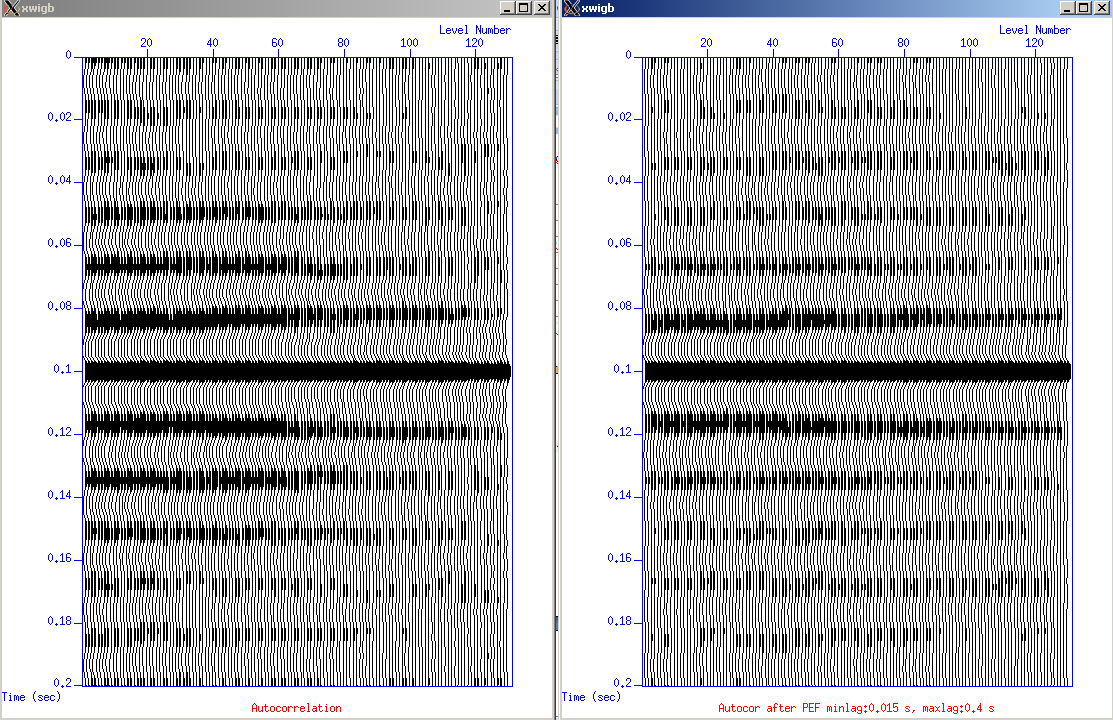
\includegraphics[width=409pt, height=265pt, keepaspectratio=true]{LatihanVSPsu-fig011.png}
%%\caption{This should be the caption for \texttt{LatihanVSPsu-fig011.png}.}
%%\end{figure}

\vspace{16pt}
\textit{Autocorrelation QC, before (left) and after PEF (right)}

\vspace{4pt}
%%\begin{figure}[htbp]
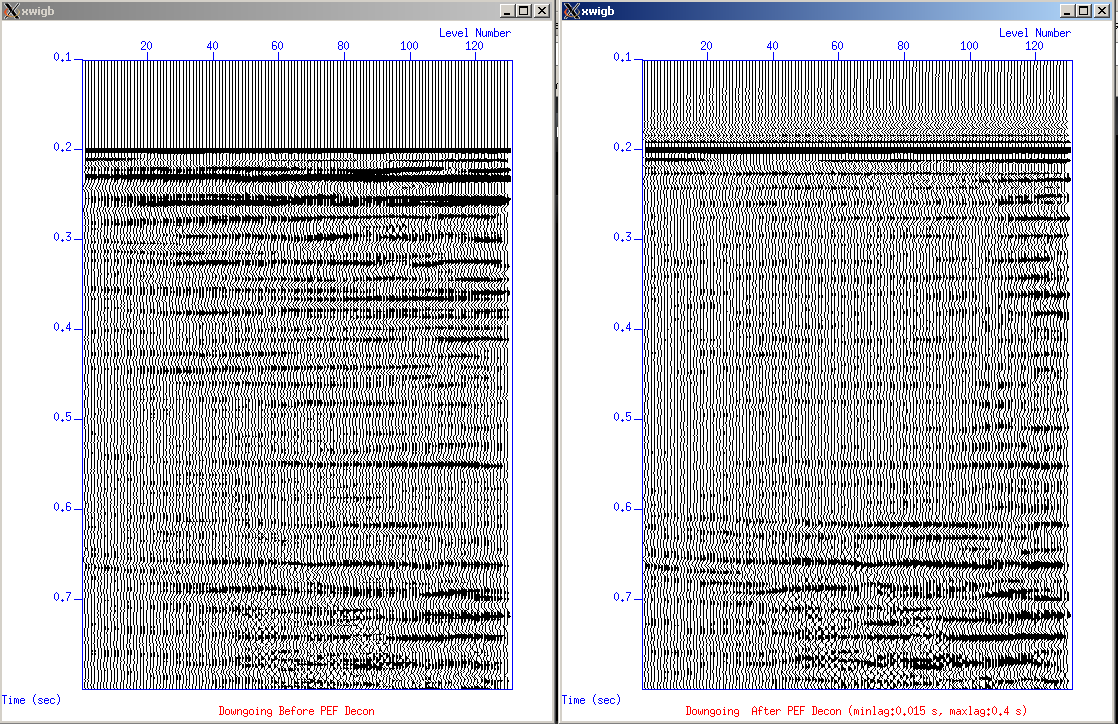
\includegraphics[width=402pt, height=261pt, keepaspectratio=true]{LatihanVSPsu-fig012.png}
%%\caption{This should be the caption for \texttt{LatihanVSPsu-fig012.png}.}
%%\end{figure}

\vspace{16pt}
\textit{Downgoing wavefield before (left) and after (right) PEF decon\pagebreak{}}
\end{center}

\vspace{16pt}
\baselineskip=12pt
\leftskip=0pt
\textbf{Script Source:}

\vspace{4pt}
Filename: CheckAutoCorrelation.sh

\vspace{4pt}
00001 \#!/bin/bash

\vspace{4pt}
00002 

\vspace{4pt}
00017 \#input

\vspace{4pt}
00018 input\_dn=velf\_dn.su

\vspace{4pt}
00019 tt=tt-header.txt

\vspace{4pt}
00020 output\_pef\_dn=pef\_dn.su

\vspace{4pt}
00021 

\vspace{4pt}
00022 \#set parameter

\vspace{4pt}
00023 minlag=0.015 \#s

\vspace{4pt}
00024 maxlag=0.4 \#s

\vspace{4pt}
00025 pnoise=0.0005

\vspace{4pt}
00026 bpf=3,5,120,140 \#4 points bandpass specification

\vspace{4pt}
00027 

\vspace{4pt}
00028 \#align downgoing

\vspace{4pt}
00029 fac=-1 \# (+1) aligned TWT upgoing , (-1) aligned downgoing

\vspace{4pt}
00030 al=200 \# 0 for TWT upgoing, 200 for aligned at 200 msec

\vspace{4pt}
00031 tmin=0

\vspace{4pt}
00032 tmax=5

\vspace{4pt}
00033 awk '\{print \$1*1000\}' \$tt \texttt{>} tt.tmp 

\vspace{4pt}
00034 a2b \texttt{<}tt.tmp \texttt{>} tt\_header.bin

\vspace{4pt}
00035 

\vspace{4pt}
00036 \#check autocorrelation before PEF

\vspace{4pt}
00037 sugain \texttt{<} \$input\_dn tpow=1 \textbar{} suacor sym=1 norm=1 \textbackslash{}

\vspace{4pt}
00038            \textbar{} suxwigb perc=95 label1=\texttt{"}Time (sec)\texttt{"} 
label2=\texttt{"}Level Number\texttt{"}  

\vspace{4pt}
\parindent=18pt
title=\texttt{"}Autocorrelation\texttt{"} wbox=550 xbox=10\&

\vspace{4pt}
\parindent=0pt
00039 \#Apply to Attack Reveberations

\vspace{4pt}
00040 supef \texttt{<} \$input\_dn minlag=\$minlag maxlag=\$maxlag pnoise=\$pnoise 
 \textbar{} 

\vspace{4pt}
sufilter f=\$bpf \texttt{>} \$output\_pef\_dn

\vspace{4pt}
00041 sugain \texttt{<} \$output\_pef\_dn tpow=1 \textbar{} suacor  sym=1 norm=1 
 \textbackslash{}

\vspace{4pt}
00042            \textbar{} suxwigb title=\texttt{"}Autocor after PEF minlag:\$minlag 
s, 

\vspace{4pt}
\parindent=18pt
maxlag:\$maxlag s\texttt{"} perc=95 label1=\texttt{"}Time (sec)\texttt{"} label2=\texttt{"}Level 
Number\texttt{"} 

\vspace{4pt}
wbox=550 xbox=570\&

\vspace{4pt}
00043 

\vspace{4pt}
00044 

\vspace{4pt}
00045 \#display pef application on downgoing signal

\vspace{4pt}
\parindent=0pt
00046 sushw \texttt{<} \$input\_dn infile=tt\_header.bin key=delrt \textbar{} suchw 
key1=delrt 

\vspace{4pt}
\parindent=18pt
key2=delrt a=\$al b=\$fac \textbackslash{}

\vspace{4pt}
\parindent=0pt
00047            \textbar{} sushift tmin=\$tmin tmax=\$tmax\textbar{}suwind tmin=0.1 
tmax=0.8\texttt{>} 

\vspace{4pt}
\parindent=18pt
\$input\_dn.align.tmp

\vspace{4pt}
\parindent=0pt
00048 sushw \texttt{<} \$output\_pef\_dn infile=tt\_header.bin key=delrt \textbar{} 
suchw 

\vspace{4pt}
key1=delrt key2=delrt a=\$al b=\$fac \textbackslash{}

\vspace{4pt}
00049            \textbar{} sushift tmin=\$tmin tmax=\$tmax\textbar{}suwind tmin=0.1 
tmax=0.8\texttt{>} 

\vspace{4pt}
\parindent=18pt
\$output\_pef\_dn.align.tmp

\vspace{4pt}
\parindent=0pt
00050 

\vspace{4pt}
00051 suxwigb \texttt{<} \$input\_dn.align.tmp perc=95 title=\texttt{"}Downgoing 
Before PEF 

\vspace{4pt}
Decon\texttt{"} label1=\texttt{"}Time (sec)\texttt{"} label2=\texttt{"}Level Number\texttt{"} 
 wbox=550 xbox=10\&

\vspace{4pt}
00052 suxwigb \texttt{<} \$output\_pef\_dn.align.tmp perc=95 title=\texttt{"}Downgoing 
 After PEF 

\vspace{4pt}
\parindent=18pt
Decon (minlag:\$minlag s, maxlag:\$maxlag s)\texttt{"}  label1=\texttt{"}Time (sec)\texttt{"} 

\vspace{4pt}
label2=\texttt{"}Level Number\texttt{"}  wbox=550 xbox=570\&

\vspace{4pt}
\parindent=0pt
00053 \pagebreak{}

\vspace{36pt}
\subsection*{{\large{}\textbf{6Deconvolution/ApplyDecon.sh File Reference}}}

\vspace{12pt}
Deconvolution/ApplyDecon.sh6Deconvolution/ApplyDecon.sh\label{AAAAAAAAAN}

\vspace{12pt}
Apply PEF to upgoing wavefield. 

\vspace{24pt}
\subsubsection*{\textbf{Detailed Description}}

\vspace{1pt}
This is sequential script after CheckAutoCorrelation.sh. In previous script we 
estimated the minlag and maxlag for downgoing wavefield. If the PEF decon is working 
as expected, we can collapse the reverberations, and the minlag \& maxlag can also 
be applied for upgoing wavefield.

\vspace{1pt}
We can apply another median filter to remove noise after predictive decon.

\vspace{4pt}
\textbf{Usage:}

\vspace{4pt}
Open the file in text editor, and edit required parameters as necessary. The parameter 
description is given here. Run the command from console. 

\vspace{4pt}
\$./ApplyDecon.sh 

\vspace{16pt}
*** Before run, please manually copy the SU file that you want to process to this 
directory, 

\vspace{4pt}
\$cp ../5Separation/velf\_up.su .

\vspace{4pt}
\$cp ../5Separation/velf\_down.su .

\vspace{4pt}
\$cp ../0ImportSEGY/tt-header.txt .

\vspace{16pt}
\textbf{Output:}

\vspace{4pt}
- SU file for upgoing after PEF decon

\vspace{4pt}
- Enhanced upgoing SU file

\vspace{4pt}
\textbf{Parameters:}

\vspace{4pt}
\textit{input\_up} Upgoing wavefield to be deconvolved 

\vspace{4pt}
\begin{tabular}{|>{\raggedright}p{54pt}|>{\raggedright}p{245pt}|}
\hline
\tabularnewline
\hline
t\textit{t}  & ASCII file of Transit Time picks data \tabularnewline
\hline
o\textit{utput\_pef\_up}  & Upgoing Wavefield after predictive decon \tabularnewline
\hline
o\textit{utput\_pef\_up\_enh}  & Enhancement of Upgoing Wavefield after predictive 
decon \tabularnewline
\hline
e\textit{nhc\_up}  & Number of median level for upgoing enhancement \tabularnewline
\hline
m\textit{inlag}  & First lag of prediction filter (sec) \tabularnewline
\hline
m\textit{axlag}  & lag \tabularnewline
\hline
p\textit{noise}  & relative additive noise level \tabularnewline
\hline
b\textit{pf}  & Four points of BPF filter \tabularnewline
\hline
\end{tabular}

\vspace{1pt}
Definition in file \textbf{ApplyDecon.sh}.

\vspace{4pt}
\textbf{Author:}

\vspace{4pt}
\leftskip=18pt
fahdi@gm2001.net 

\vspace{4pt}
\leftskip=0pt
\textbf{Date:}

\vspace{4pt}
\leftskip=18pt
February 2012 

\vspace{16pt}
\leftskip=0pt
\textbf{Output Example:}

\vspace{4pt}
\$./ApplyDecon.sh \&

\vspace{16pt}
\begin{center}
%%\begin{figure}[htbp]
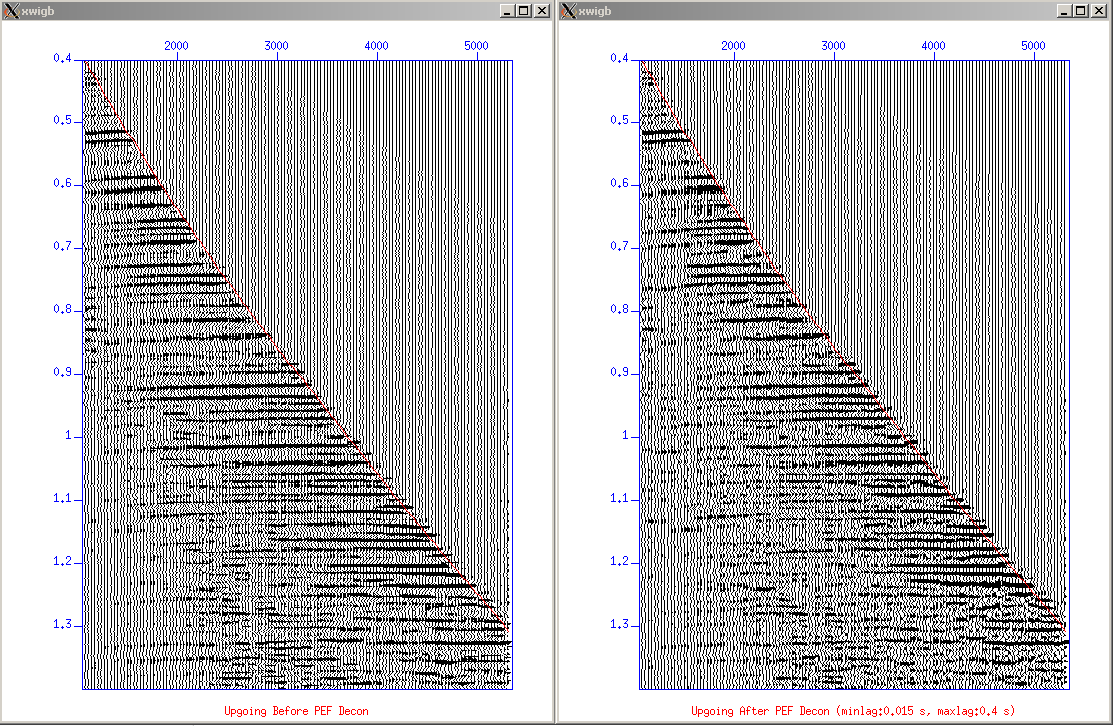
\includegraphics[width=409pt, height=267pt, keepaspectratio=true]{LatihanVSPsu-fig013.png}
%%\caption{This should be the caption for \texttt{LatihanVSPsu-fig013.png}.}
%%\end{figure}

\vspace{16pt}
\textit{Upgoing wavefield before decon (left) and after decon (right)}

\vspace{16pt}
%%\begin{figure}[htbp]
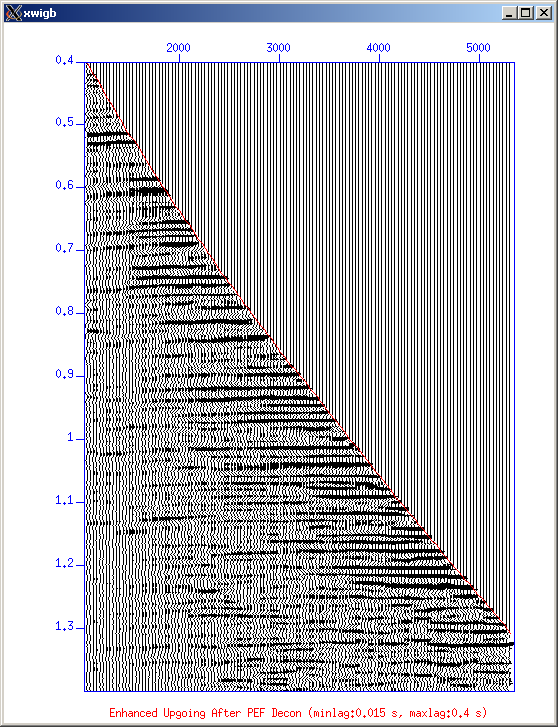
\includegraphics[width=230pt, height=300pt, keepaspectratio=true]{LatihanVSPsu-fig014.png}
%%\caption{This should be the caption for \texttt{LatihanVSPsu-fig014.png}.}
%%\end{figure}

\vspace{16pt}
\textit{Enhanced Deconvolved upgoing wavefield\pagebreak{}}
\end{center}

\vspace{16pt}
\baselineskip=12pt
\leftskip=0pt
\textbf{Script Source:}

\vspace{4pt}
Filename: ApplyDecon.sh

\vspace{16pt}
00001 \#!/bin/bash

\vspace{4pt}
00002 

\vspace{4pt}
00020 \#input

\vspace{4pt}
00021 input\_up=velf\_up.su

\vspace{4pt}
00022 tt=tt-header.txt

\vspace{4pt}
00023 output\_pef\_up=pef\_up.su

\vspace{4pt}
00024 output\_pef\_up\_enh=pef\_up\_enh.su

\vspace{4pt}
00025 enhc\_up=5

\vspace{4pt}
00026 

\vspace{4pt}
00027 \#set parameter

\vspace{4pt}
00028 minlag=0.015 \#s

\vspace{4pt}
00029 maxlag=0.4 \#s

\vspace{4pt}
00030 pnoise=0.0005

\vspace{4pt}
00031 bpf=3,5,120,140 \#4 points bandpass specification

\vspace{4pt}
00032 

\vspace{4pt}
00033 \#housekeeping-start

\vspace{4pt}
00034 awk '\{print \$1*0+0.200,\$2\}' \$tt \texttt{>} minustt.tmp

\vspace{4pt}
00035 awk '\{print \$1*2,\$2\}' \$tt \texttt{>} twt.tmp

\vspace{4pt}
00036 

\vspace{4pt}
00037 \#align 

\vspace{4pt}
00038 fac=1 \# (+1) aligned TWT upgoing , (-1) aligned downgoing

\vspace{4pt}
00039 al=0 \# 0 for TWT upgoing, 200 for aligned at 200 msec

\vspace{4pt}
00040 tmin=0

\vspace{4pt}
00041 tmax=5

\vspace{4pt}
00042 awk '\{print \$1*1000\}' \$tt \texttt{>} tt.tmp 

\vspace{4pt}
00043 a2b \texttt{<}tt.tmp \texttt{>} tt\_header.bin

\vspace{4pt}
00044 

\vspace{4pt}
00045 

\vspace{4pt}
00046 nrec=(\$(wc -l \$tt \textbar{} awk '\{print \$1\}')) \#housekeeping

\vspace{4pt}
00047 

\vspace{4pt}
00048 \#apply enhancement to pef up

\vspace{4pt}
00049 awk '\{print \$2\}' \$tt \texttt{>} xfile.tmp

\vspace{4pt}
00050 a2b \texttt{<} xfile.tmp n1=\$nrec\texttt{>} xfile.bin

\vspace{4pt}
00051 

\vspace{4pt}
00052 awk '\{print \$1\}' \$tt \texttt{>} tfile.tmp

\vspace{4pt}
00053 a2b \texttt{<} tfile.tmp n1=\$nrec\texttt{>} tfile.bin

\vspace{4pt}
00054 \#housekeeping-end

\vspace{4pt}
00055 

\vspace{4pt}
00056 \#check autocorrelation before PEF

\vspace{4pt}
00057 \#sugain \texttt{<} \$input\_up tpow=1 \textbar{} suacor sym=1 norm=1 \textbackslash{}

\vspace{4pt}
00058 \#          \textbar{} suxwigb perc=95 label1=\texttt{"}Time (sec)\texttt{"} 
label2=\texttt{"}Level Number\texttt{"}  

\vspace{4pt}
title=\texttt{"}Autocorrelation\texttt{"} \&

\vspace{4pt}
00059 

\vspace{4pt}
00060 \#Apply PEF

\vspace{4pt}
00061 supef \texttt{<} \$input\_up minlag=\$minlag maxlag=\$maxlag pnoise=\$pnoise 
 \textbar{} 

\vspace{4pt}
sufilter f=\$bpf \texttt{>} \$output\_pef\_up

\vspace{4pt}
00062 \#sugain \texttt{<} \$output\_pef\_up tpow=1 \textbar{} suacor  sym=1 norm=1 
 \textbackslash{}

\vspace{4pt}
00063 \#          \textbar{} suxwigb title=\texttt{"}Autocor after PEF minlag:\$minlag 
s, 

\vspace{4pt}
maxlag:\$maxlag s\texttt{"} perc=95 \&

\vspace{4pt}
00064 

\vspace{4pt}
00065 sumedian \texttt{<} \$output\_pef\_up xfile=xfile.bin tfile=tfile.bin key=gelev 

\vspace{4pt}
\parindent=18pt
nshift=\$nrec subtract=0 median=1 nmed=\$level\_up sign=+1 \textbackslash{}

\vspace{16pt}
\parindent=0pt
00066            \textbar{} sumute key=gelev nmute=\$nrec xfile=xfile.bin 

\vspace{4pt}
tfile=tfile.bin mode=0 \texttt{>} \$output\_pef\_up\_enh

\vspace{4pt}
00067 

\vspace{4pt}
00068 \#display pef application on upgoing signal

\vspace{4pt}
00069 sushw \texttt{<} \$input\_up infile=tt\_header.bin key=delrt \textbar{} suchw 
key1=delrt 

\vspace{4pt}
\parindent=18pt
key2=delrt a=\$al b=\$fac \textbackslash{}

\vspace{4pt}
\parindent=0pt
00070            \textbar{} sushift tmin=\$tmin tmax=\$tmax\textbar{}suwind tmin=0 
tmax=\$tmax\texttt{>} 

\vspace{4pt}
\parindent=18pt
\$input\_up.align

\vspace{4pt}
\parindent=0pt
00071 sushw \texttt{<} \$output\_pef\_up infile=tt\_header.bin key=delrt \textbar{} 
suchw key1=delrt 

\vspace{4pt}
\parindent=18pt
key2=delrt a=\$al b=\$fac \textbackslash{}

\vspace{4pt}
\parindent=0pt
00072            \textbar{} sushift tmin=\$tmin tmax=\$tmax\textbar{}suwind tmin=0 
tmax=\$tmax\texttt{>} 

\vspace{4pt}
\parindent=18pt
\$output\_pef\_up.align

\vspace{4pt}
\parindent=0pt
00073 sushw \texttt{<} \$output\_pef\_up\_enh infile=tt\_header.bin key=delrt \textbar{} 
suchw 

\vspace{4pt}
\parindent=18pt
key1=delrt key2=delrt a=\$al b=\$fac \textbackslash{}

\vspace{4pt}
\parindent=0pt
00074            \textbar{} sushift tmin=\$tmin tmax=\$tmax\textbar{}suwind tmin=0 
tmax=\$tmax\texttt{>} 

\vspace{4pt}
\parindent=18pt
\$output\_pef\_up\_enh.align

\vspace{4pt}
\parindent=0pt
00075 

\vspace{4pt}
00076 suwind \texttt{<} \$input\_up.align tmin=0.4 tmax=1.4 \textbar{} suxwigb 
perc=95 

\vspace{4pt}
title=\texttt{"}Upgoing  Before PEF Decon\texttt{"} key=gelev curve=twt.tmp npair=\$nrec,1 

\vspace{4pt}
curvecolor=red \&

\vspace{4pt}
00077 suwind \texttt{<} \$output\_pef\_up.align tmin=0.4 tmax=1.4 \textbar{} suxwigb 
perc=95 

\vspace{4pt}
\parindent=18pt
title=\texttt{"}Upgoing After PEF Decon (minlag:\$minlag s, maxlag:\$maxlag s)\texttt{"} 
 

\vspace{4pt}
key=gelev curve=twt.tmp npair=\$nrec,1 curvecolor=red \&

\vspace{4pt}
00078 suwind \texttt{<} \$output\_pef\_up\_enh.align tmin=0.4 tmax=1.4 \textbar{} 
suxwigb perc=95 

\vspace{4pt}
\parindent=36pt
title=\texttt{"}Enhanced Upgoing After PEF Decon (minlag:\$minlag s, \textbackslash{}

\vspace{4pt}
\parindent=0pt
maxlag:\$maxlag  s)\texttt{"}  key=gelev curve=twt.tmp npair=\$nrec,1 

\vspace{4pt}
curvecolor=red \&

\vspace{4pt}
00079 

\vspace{4pt}
00080 \#clean up

\vspace{4pt}
00081 \#rm *.bin

\vspace{4pt}
00082 \#rm *.tmp\newpage

\newpage
\vspace{12pt}
\subsection*{{\large{}\textbf{7CorrStack/CorridorStack.sh File Reference}}}

\vspace{12pt}
27CorrStack/CorridorStack.sh7CorrStack/CorridorStack.sh\label{AAAAAAAAAP}

\vspace{12pt}
Create corridor stack. 

\vspace{24pt}
\subsubsection*{\textbf{Detailed Description}}

\vspace{1pt}
The final process for Zero Offset VSP processing is creating corridor stack, that 
representing the 1-D seismic response in the borehole. This is done by taking a 
short window around transit time, and stacks it. 

\vspace{1pt}
The corridor window don't be too short, because it may not capture the amplitude 
variation, but also not too long, because we can include multiple in the stacking 
process. 

\vspace{1pt}
For reflection below TD, we include number of traces (defined by except\_last\_trace) 
to be stack for all window.

\vspace{16pt}
\textbf{Usage:}

\vspace{4pt}
Open the file in text editor, and edit required parameters as necessary. The parameter 
description is given here. Run the command from console. 

\vspace{4pt}
\$./ApplyDecon.sh 

\vspace{16pt}
*** Before run, please manually copy the SU file that you want to process to this 
directory 

\vspace{4pt}
\$cp ../5Separation/pef\_up\_enh.su.align .

\vspace{4pt}
\$cp ../0ImportSEGY/tt-header.txt .

\vspace{4pt}
\textbf{Output:}

\vspace{4pt}
- Corridor Stack

\vspace{4pt}
\textbf{Parameters:}

\vspace{4pt}
\textit{input\_decon\_enh\_up} Input is final upgoing wavefield (after decon) 

\vspace{4pt}
\begin{tabular}{|>{\raggedright}p{54pt}|>{\raggedright}p{245pt}|}
\hline
\tabularnewline
\hline
o\textit{utput\_cstack}  & Corridor Stack Output \tabularnewline
\hline
t\textit{t}  & ASCII file of Transit Time picks data \tabularnewline
\hline
\end{tabular}

\vspace{1pt}
Definition in file \textbf{CorridorStack.sh}.

\vspace{4pt}
\textbf{Author:}

\vspace{4pt}
\leftskip=18pt
fahdi@gm2001.net 

\vspace{4pt}
\leftskip=0pt
\textbf{Date:}

\vspace{4pt}
\leftskip=18pt
February 2012 

\vspace{4pt}
\leftskip=0pt
\textbf{Output Example:}

\vspace{4pt}
\$./CorridorStack.sh \&

\vspace{16pt}
%%\begin{figure}[htbp]
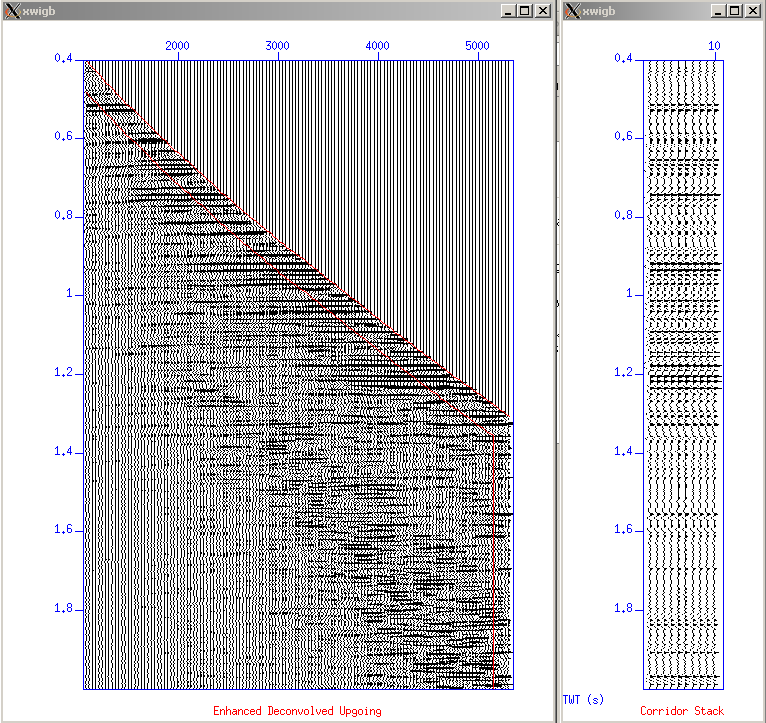
\includegraphics[width=465pt, height=439pt, keepaspectratio=true]{LatihanVSPsu-fig015.png}
%%\caption{This should be the caption for \texttt{LatihanVSPsu-fig015.png}.}
%%\end{figure}

\vspace{16pt}
\begin{center}
\textit{Upgoing wavefield and 1-D corridor stack repeated 12 times\pagebreak{}}
\end{center}

\vspace{4pt}
\baselineskip=12pt
\leftskip=0pt
\textbf{Script Source:}

\vspace{4pt}
Filename: ApplyDecon.sh

\vspace{16pt}
00001 \#!/bin/bash

\vspace{4pt}
00002 

\vspace{4pt}
00014 \#input

\vspace{4pt}
00015 input\_decon\_enh\_up=pef\_up\_enh.su.align

\vspace{4pt}
00016 output\_cstack=corr\_stack.su

\vspace{4pt}
00017 tt=tt-header.txt

\vspace{4pt}
00018 

\vspace{4pt}
00019 \#set parameter

\vspace{4pt}
00020 corridor=0.08 \#s

\vspace{4pt}
00021 except\_last\_trace=5;

\vspace{4pt}
00022 

\vspace{4pt}
00023 \#housekeeping

\vspace{4pt}
00024 nrec=(\$(wc -l \$tt \textbar{} awk '\{print \$1\}')) \#housekeeping

\vspace{4pt}
00025 last\_rec=\$((\$nrec - \$except\_last\_trace))

\vspace{4pt}
00026 

\vspace{4pt}
00027 awk -v corridor=\$corridor -v last\_rec=\$last\_rec \textbackslash{}

\vspace{4pt}
00028            'BEGIN \{i=1\}\{if (i\texttt{<}=last\_rec)\{print ((\$1*2)+corridor), 
\$2\} 

\vspace{4pt}
else \{print 9,\$2\} i++\}' \$tt \textbackslash{}

\vspace{4pt}
00029            \textbar{} awk '\{ printf \texttt{"}\%4f \%d\textbackslash{}n\texttt{"}, 
\$1, \$2 \}' \texttt{>} \$tt.inside 

\vspace{4pt}
00030 

\vspace{4pt}
00031 awk '\{ printf \texttt{"}\%4f \%d\textbackslash{}n\texttt{"}, \$1*2, \$2 
\}' \$tt \texttt{>} \$tt.outside

\vspace{4pt}
00032 

\vspace{4pt}
00033 \#apply enhancement to pef up

\vspace{4pt}
00034 awk '\{print \$2\}' \$tt \texttt{>} xfile.tmp

\vspace{4pt}
00035 a2b \texttt{<} xfile.tmp n1=\$nrec\texttt{>} xfile.bin

\vspace{4pt}
00036 

\vspace{4pt}
00037 awk '\{print \$1\}' \$tt.inside \texttt{>} tfile.inside.tmp

\vspace{4pt}
00038 a2b \texttt{<} tfile.inside.tmp n1=\$nrec\texttt{>} tfile.inside.bin

\vspace{4pt}
00039 

\vspace{4pt}
00040 awk '\{print \$1\}' \$tt.outside \texttt{>} tfile.outside.tmp

\vspace{4pt}
00041 a2b \texttt{<} tfile.outside.tmp n1=\$nrec\texttt{>} tfile.outside.bin

\vspace{4pt}
00042 

\vspace{4pt}
00043 \#housekeeping-end

\vspace{4pt}
00044 

\vspace{4pt}
00045 \#display corridor window

\vspace{4pt}
00046 suwind \texttt{<} \$input\_decon\_enh\_up tmin=0.4 tmax=2.0 \textbar{} suxwigb 
perc=95 

\vspace{4pt}
\parindent=18pt
title=\texttt{"}Enhanced Deconvolved Upgoing\texttt{"}  key=gelev 

\vspace{4pt}
curve=\$tt.inside,\$tt.outside npair=\$nrec,\$nrec curvecolor=red \&

\vspace{4pt}
00047 

\vspace{4pt}
00048 \#mute, change word, stack

\vspace{4pt}
\parindent=0pt
00049 sumute \texttt{<} \$input\_decon\_enh\_up key=gelev nmute=\$nrec xfile=xfile.bin 

\vspace{4pt}
\parindent=18pt
tfile=tfile.inside.bin mode=1 \textbackslash{}

\vspace{4pt}
\parindent=0pt
00050            \textbar{} sustack repeat=12 normpow=1.0 \texttt{>} \$output\_cstack

\vspace{4pt}
00051 \#display   

\vspace{4pt}
00052 suwind \texttt{<}  \$output\_cstack tmin=0.4 tmax=2.0 \textbackslash{}

\vspace{4pt}
00053            \textbar{} suxwigb perc=99 xbox=610 wbox=200 label1='TWT (s)' 

\vspace{4pt}
\parindent=18pt
title='Corridor Stack'\&

\vspace{4pt}
\parindent=0pt
00054 

\vspace{4pt}
00055 \#clean up

\vspace{4pt}
00056 rm *.tmp

\vspace{4pt}
00057 \pagebreak{}

\vspace{12pt}
\subsection*{{\large{}\textbf{Reference}}}

\vspace{12pt}
Seismic Unix CWP 

\vspace{12pt}
Ela2D

\vspace{36pt}
\subsection*{{\large{}\textbf{Acknowledgment}}}

\vspace{12pt}
Thanks to Sunawar Kunaifi ({\color{color02} \emph{sunawar.kunaifi@gmail.com}}) 
for interesting discussion SeismicUnix application for VSP.

\vspace{24pt}
Thanks to DCS Schlumberger Indonesia for help and support.

\newpage

\end{document}
